\documentclass[output=paper]{langscibook} 


\author{Barbara Tomaszewicz-Özakın\affiliation{University of Cologne}}
\title{\textit{Some}, \textit{most}, \textit{all} in a visual world study}  
\abstract{In a visual world eye-tracking study I find that Polish quantifiers \textit{niektóre} `some', \textit{większość} `most of', \textit{najwięcej} `the most' and \textit{wszystkie} `all' elicit distinctive patterns of looks, consistent with their semantics. \textit{Niektóre} `some' has a strong scalar implicature: the meaning `some-not-all' is processed immediately as the quantifier is heard. The superlative \textit{najwięcej} `the most' quickly triggers comparisons between the target and the other sets. The proportional \textit{większość} `most of' elicits a pattern suggesting that its verification involves the estimation of the total set. With \textit{wszystkie} `all'  the identification of the target set is the fastest.


\keywords{quantifiers, semantics–cognition interface, eye-tracking, Polish}}

\begin{document}
\SetupAffiliations{mark style=none}
\maketitle

\section{Introduction: Interpreting quantifiers} 

We talk about quantities all the time while describing the world. Quantifiers are natural language expressions used to
describe quantities with or without using number terms. Semantically they express relations between sets \citep{barwise1981generalized}, e.g., \textit{most of }in the sentence \textit{Most of the balls are blue} tells us that the set of
balls that are blue is larger than the set of non-blue balls. We can easily assess the conditions that make this
sentence true/false, but how do we verify such sentences in real-life situations? The generalized quantifier theory
\citep{mostowski1960generalization, perlindstrom1966first,montague1973proper} is silent about this issue, mainly because for philosophers (\citealt{montague1973proper}, a.o.) semantics was a branch of mathematics and not of psychology \citep{partee2011formal}. Psychologists, however, have long been
studying the number sense in humans, a dedicated brain system for abstract representation of number and the source of
our mathematical intuitions, which is employed in the judgments involving quantifiers \citep{feigenson2004core,mcmillan2005neural,mcmillan2006quantifier,clark2007number,dehaene2009origins,dehaene2011number,troiani2009logical}. Speakers have different ways of referring to quantities:
number terms when the specific size of the set is at issue, and vague quantifiers like \textit{some} and \textit{most}
or context-dependent quantifiers like \textit{few} and \textit{many}, when they refer to approximate quantities. The
present study addresses two critical questions about quantifiers: (i) what is included in the lexical representation of quantifier meanings
and (ii) what the psychological mechanisms involved in the interpretation of those meanings are.

Investigating those two questions, \citet{pietroski2009meaning} and \citet{lidz2011interface} put forth a novel hypothesis that what
participants are doing to verify sentences containing quantifiers, i.e., (ii), can be directly determined by quantifier
semantics, (i). To illustrate, in order to verify that most balls are blue we need to compare the numbers of
blue and and non-blue balls, but how do we obtain the number of non-blue balls? If there are balls in one other color,
we can simply count them. If there are more colors, we can count the numbers of balls in each other color and add them
up; or we can obtain the number of all balls and subtract the number of the blue balls from it; or we can instead
verify if blue balls are more than the half of all balls. But do we even need to count? Children who are not yet able
to count are perfectly able to understand sentences containing \textit{most} \citep{halberda2008development,odic2018individuals}, and in real-life situations we do not need to know precise quantities to use \textit{most}.\largerpage

\citet{pietroski2009meaning, bates2015parsimonious, tomaszewicz2011verification, tomaszewicz2012semantics, tomaszewicz2013linguistic, tomaszewicz2018focus, hunter2017verification, Knowlton2021} obtained experimental evidence that \textit{most of} induces a subconscious choice of a procedure based on subtraction for
verification against visual displays, even in situations where comparing the numerosity of the target set and one other
set directly would be more efficient. Why would the mind not subconsciously choose the most efficient procedure in a
given situation? According to the hypothesis it is because the mind follows the “instructions” encoded in the logical
function representing the meaning of a quantifier. \citet{tomaszewicz2011verification, tomaszewicz2012semantics, tomaszewicz2013linguistic, tomaszewicz2018focus} showed that, in contrast to the proportional quantifier \textit{most of} (Polish \textit{większość}), the superlative \textit{najwięcej} `the most',
as in \textit{Najwięcej kulek jest niebieskich} `Blue balls are more numerous than balls in any other color', directs
participants’ subconscious attention to obtaining the numerosities of each other color set. The participants were
prompted to switch between verification procedures by a change in the linguistic input, but not by a change in the
visual input. Thus, the motivation for the subconscious switch in procedures is not to maximize efficiency.
Participants used the procedure associated with each quantifier, and in effect, the same display was verified
differently depending on which information the visual system was instructed to use by the lexical representation of
quantifier meanings.

The present experiment was designed to uncover the details of the lexical semantic specification of the Polish
quantifiers \textit{niektóre} `some' and \textit{większość} `most of' in comparison to
\textit{wszystkie} `all' and \textit{najwięcej} `the most'. It utilizes eye-movement as a
representational measure in the visual world paradigm. Visual world eye-tracking has been used to demonstrate how
comprehenders rapidly integrate different sources of information in order to identify the referents in the visual
display as the sentence unfolds over time (\citealt{tanenhaus1995integration, allopenna1998tracking}). The visual world
paradigm allows for the closest approximation of real-life visual contexts in an experimental setting. Our conscious
experience is that our eyes glide from one thing to another thing, but, in fact, unless we are tracking a moving object, our eyes
perceive images in a series of rapid jerky movements (saccades). We can track the series of fixations at a particular
point and the saccades away from that point in order to analyze which parts of the image attract attention and how. In
a visual world task, participants hear the sentence as they inspect the visual scene and their eye movements are
recorded; in particular, the proportion of looks to the target in the picture is measured. This makes it an excellent
tool for the investigation of incremental processing. At the point in the sentence when the quantifier is heard,
participants’ subconscious attention should be directed to different aspects of the scene, towards or away from the
target, depending on the semantics of the quantifier.

In the current experiment, the four Polish quantifiers, \textit{wszystkie} `all', \textit{niektóre} `some', \textit{większość} `most of' (proportional \textit{most}), and \textit{najwięcej} `the most' (superlative \textit{most}, henceforth \textit{most\textsc{-sup}}), appeared in the same carrier
sentence, describing the same identical display for \textit{some}, \textit{most of} and \textit{most\textsc{-sup}} (screens for \textit{all} needed to differ as will be explained shortly). I employed the gumball paradigm of \citet{degen2011making,degen2016availability}. Participants evaluated sentences of the form ‘You got all/some/most
of/most\textsc{-sup} blue balls’ against displays of a ball machine dispensing balls of three colors from upper to lower chambers; see \figref{tom:fig:machine}. The correlate of the processing of the information about the quantifier semantics was the proportion of looks to the target (the set of blue balls) vs. the so-called distractors (the two other color sets).

%\bigskip

% \begin{center}
% \tablefirsthead{}
% \tablehead{}
% \tabletail{}
% \tablelasttail{}
% \begin{supertabular}{m{6cm}m{0.5cm}m{6cm}}
%  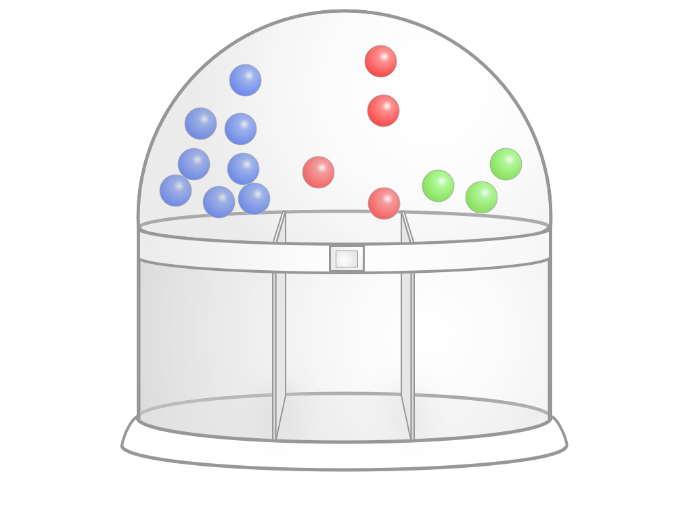
\includegraphics[width=7cm]{draftsinfonijarevisedfinal1-img001.png}  &
% ~

% ~

% ~

% ~

% \textcolor[rgb]{0.5019608,0.5019608,0.5019608}{→ }

% ~
%  &
%  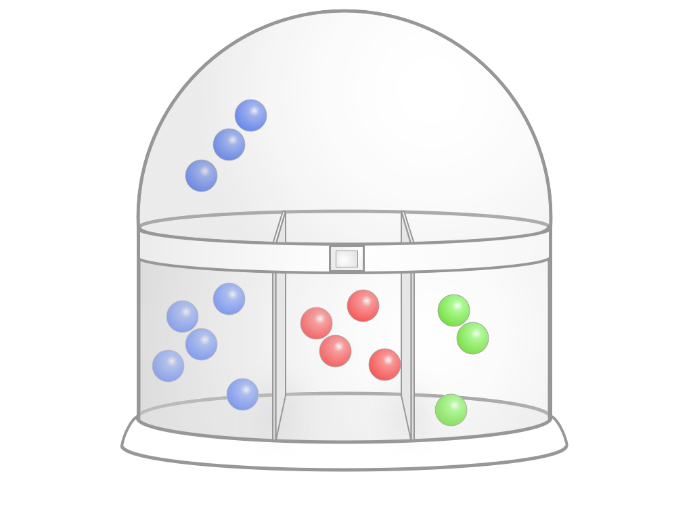
\includegraphics[width=7cm]{draftsinfonijarevisedfinal1-img002.png} \\
% The ball machine at the beginning of the trial. &
% ~
%  &
% After a button press, the machine dispenses balls to the lower chambers and after 500ms the stimulus sentence is
% played.\\
% \end{supertabular}
% \end{center}
% \begin{figure}[h]
% \centering
%     \caption{The blue set is the target.}
%     \label{tom:fig:machine}
% \end{figure}


%\bigskip


\begin{figure}\small
    \begin{tikzpicture}
\node(img1) [text width=5cm]{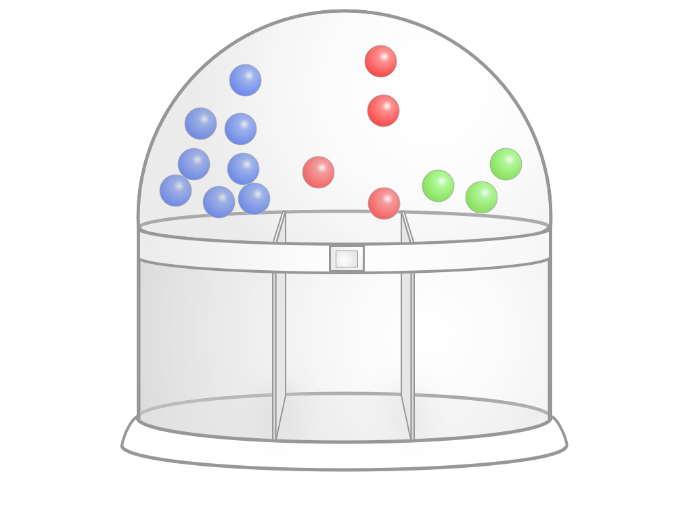
\includegraphics[width=\textwidth]{draftsinfonijarevisedfinal1-img001.png}} ;
\node(img2) [text width=5cm,right = 1cm of img1] {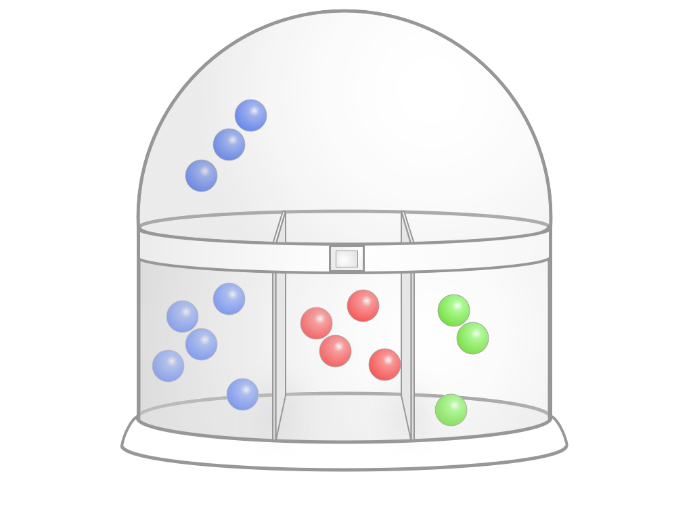
\includegraphics[width=\textwidth]{draftsinfonijarevisedfinal1-img002.png}} ;
\node[text width=5cm,below=1mm of img1] {%\raggedright
The ball machine at the beginning of the trial};
\node[text width=5cm,below=1mm of img2] {%\raggedright
After a button press, the machine dispenses balls to the lower chambers and after 500\,ms the stimulus sentence is
played};
\draw[->,thick] (img1) -- (img2);
\end{tikzpicture}
\caption{The blue set is the target.}
    \label{tom:fig:machine}
\end{figure}

I thus build on the results of \citet{huang2009online, huang2011logic, grodner2010some, degen2011making, degen2016availability}, who showed that contextual effects on the interpretation of quantifiers are reflected in eye-movement patterns. Those
studies investigated the time course of scalar implicatures, i.e., the pragmatic aspects of the meaning of the quantifier
\textit{some}, while I concentrate on the precise semantic distinctions between the four Polish quantifiers to test
both the scalar implicature of Polish \textit{niektóre} `some' \citep{spychalska-msc} and the verification procedure associated
with Polish \textit{większość} `most of' \citep{szymanik2010comprehension}. The results of the visual verification experiments (visual search
paradigm) in 
\citet{pietroski2009meaning}, \citet{lidz2011interface}, \citet{tomaszewicz2011verification, tomaszewicz2012semantics, tomaszewicz2013linguistic}, \citet{hunter2017verification}, and \citet{Knowlton2021} indicate that quantifier
semantics guides the subconscious adoption of a verification strategy. The visual search paradigm involves comparisons
of the accuracy of judgments with reference to rapidly presented displays (200--300\,ms), i.e., accuracy is taken as a
proxy for the processing cost. In these prior experiments the number of different color sets affected accuracy in different
ways depending on the quantifier in the stimulus sentence. So while in the visual search paradigm it is assumed that
the sentence stimulus somehow provides an instruction for verification, the visual world paradigm in the current
study enables us to tap into the real-time construction of this instruction as the auditory stimulus unfolds.\footnote{See
\citet{huettig2011looking} for an argument how the two paradigms, visual world and visual search, provide converging evidence
for the role of working memory in the interactions between linguistic input and visual attention.}


%\bigskip


%\bigskip

\section{The current study} 
\subsection{Methods} \label{tom:Methods}

In each trial (72 trials in 3 blocks of 24), participants ($n=35$), saw a fixation cross and the display of a
ball dispensing machine with its upper chambers filled with 3 colors of balls (bottom chambers empty), as in the left panel of \figref{tom:fig:machine}. After 2 seconds, the button in the center of the machine turned yellow, and the participants clicked on the
button. Upon clicking, a grey mask was displayed for 200\,ms. (Clicking the central button ensured that the participants were
looking at the central fixation point at the time of the auditory stimulus onset.) Now the second display was shown: the
ball machine was redisplayed with a certain number of balls of each color having dropped to the lower chamber,
e.g., right panel in \figref{tom:fig:machine}. 

After 500\,ms, the participants heard one of the stimulus sentences in \REF{tom:ex:dostales}. Their task was to click on that lower chamber
which contained the balls mentioned in the statement if they thought the statement was true, and click on the central
button otherwise.


%\bigskip

\ea\gll Dostałeś\dots\\
got.\textsc{past.2sg}\\
\glt `You got\dots'\label{tom:ex:dostales}
\ea \gll większość \minsp{\{} niebieskich / czerwonych / zielonych\} kulek.\\
most.of {} blue {} red {} green balls\\\hfill \textsc{most-of}
\glt `most of the blue/red/green balls.'
\ex \gll najwięcej \minsp{\{} niebieskich / czerwonych / zielonych\}
kulek.\\
most\textsc{-sup} {} blue {} red {} green balls\\\hfill \textsc{most\textsubscript{sup}}
\glt `the most blue/red/green balls.'
\ex \gll niektóre \minsp{\{} niebieskie {} czerwone {} zielone\} kulki.\\
some {} blue {} red {} green balls\\\hfill \textsc{some}
\glt `some blue/red/green balls.'
\ex \gll wszystkie \minsp{\{} niebieskie / czerwone / zielone\} kulki.\\
some {} blue {} red {} green balls\\\hfill \textsc{all}
\glt `all of the blue/red/green balls.'
\z
\z

\noindent All the sound files were cross-spliced and normalized using Praat Vocal Toolkit \citep{praatvocaltoolkit} so that all the quantifiers and color expressions had the same duration. Once the participants clicked indicating their response, a grey screen was
displayed for 1s and the experiment advanced to the next trial. Participants’ eye movements were recorded with an
Eyelink 1000 eye-tracker at a sampling rate of 1000\,Hz.

There were 8 conditions: 4 quantifiers (\textsc{some}/\textsc{most-of}/\textsc{most\textsubscript{sup}}\textsc{/all}) * 2 display types
(\textsc{early}/\textsc{late}). In \textsc{early} trials there was only one partitioned set, e.g. the blue set in \figref{tom:fig:machine}. In \textsc{late} trials all sets
were partitioned. The difference between the \textsc{early} and \textsc{late} displays is discussed and illustrated with pictures in the
next section (\figref{tom:fig:early}). The displays for the test sentences for the analysis of eye-movements required a Yes response.
Filler trials, half of all trials, required a No response. For Yes responses participants clicked the chamber that
matched the sentence, for No responses they clicked the button. Following \citet{degen2011making,degen2016availability}  I included what they call \textsc{garden-path} trials among the fillers in order to force the participants to pay attention and notice
that the sentences throughout the experiment might not always be true. On these trials, one set was partitioned
allowing an anticipation of a quantifier, but as the sentence unfolded it turned out this set did not match the
sentence (leading to a garden-path-like effect where you had to revise your search for
the target); see \figref{tom:fig:garden}.

\begin{figure}[h]
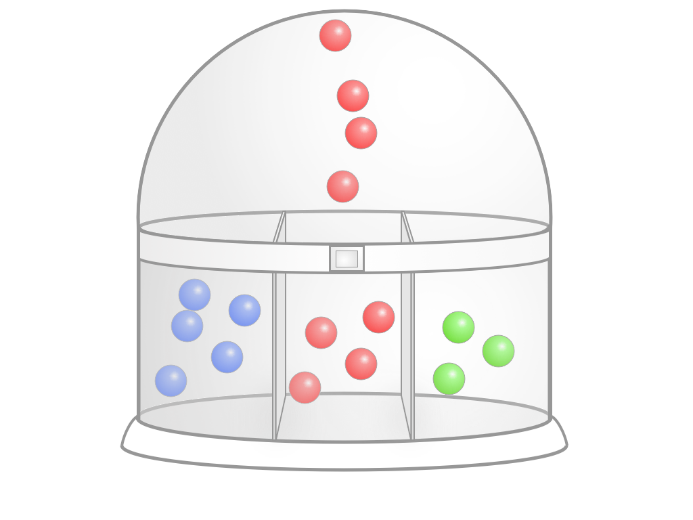
\includegraphics[width=7cm]{draftsinfonijarevisedfinal1-img003.png}
\centering
    \caption{\textsc{garden-path} condition}
    \label{tom:fig:garden}
\end{figure}

The displays were identical for 3 quantifiers: \textit{some}, \textit{most of, most}\textsc{-sup}. The quantifier
\textit{all} had different displays, because the top chamber for that color had to be empty, \figref{tom:fig:all}.


%\bigskip

%\clearpage
%\bigskip
%\bigskip

% \begin{flushleft}
% \tablefirsthead{}
% \tablehead{}
% \tabletail{}
% \tablelasttail{}
% \begin{supertabular}{m{4cm}m{4cm}m{4cm}}
%  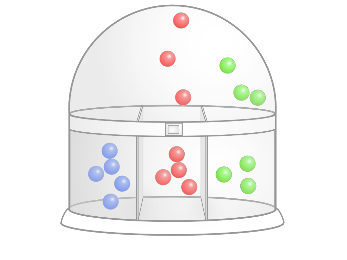
\includegraphics[width=1.5752in,height=1.1811in]{draftsinfonijarevisedfinal1-img004.png}  &
%  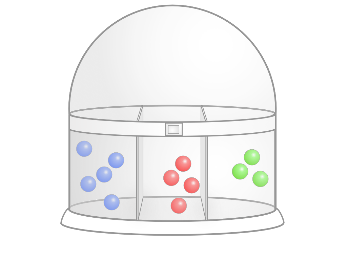
\includegraphics[width=1.5752in,height=1.1811in]{draftsinfonijarevisedfinal1-img005.png}  &
%  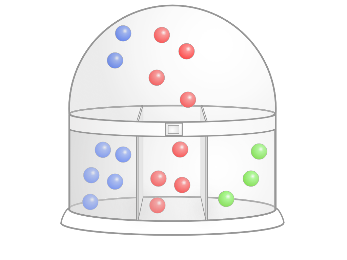
\includegraphics[width=1.5752in,height=1.1811in]{draftsinfonijarevisedfinal1-img006.png} \\
% \textit{all}{}-EARLY &
% \textit{all}{}-LATE &
% \textit{all}{}-GARDEN-PATH\\
% \end{supertabular}
% \end{flushleft}
% \begin{figure}[h]
% \centering
%     \caption{The displays for the ALL condition}
%     \label{tom:fig:all}
% \end{figure}


% \begin{figure} 
%     \begin{tikzpicture}
% \node(img1) [text width=3.5cm]{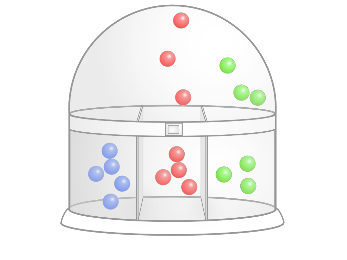
\includegraphics[width=\textwidth]{draftsinfonijarevisedfinal1-img004.png}} ;
% \node(img2) [text width=3.5cm,right = 0.6cm of img1] {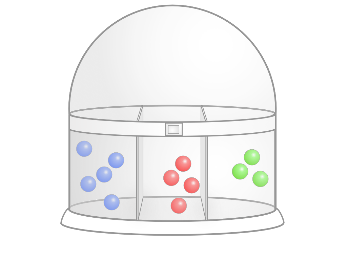
\includegraphics[width=\textwidth]{draftsinfonijarevisedfinal1-img005.png}} ;
% \node(img3) [text width=3.5cm,right = 0.6cm of img2] {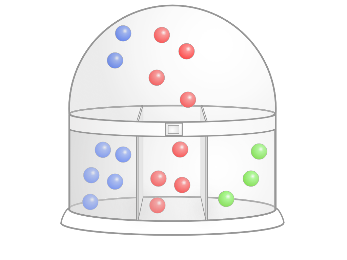
\includegraphics[width=\textwidth]{draftsinfonijarevisedfinal1-img006.png}} ;

% \node[text width=3.5cm,below=5mm of img1] {%\raggedright
% \textit{all}{}-EARLY};
% \node[text width=3.5cm,below=5mm of img2] {%\raggedright
% \textit{all}{}-LATE};
% \node[text width=3.5cm,below=5mm of img3] {%\raggedright
% \textit{all}{}-GARDEN-PATH};

% \end{tikzpicture}
% \caption{Caption}
%     \label{tom:fig:all}
% \end{figure}

\begin{figure}[h]\small
\begin{tabularx}{\textwidth}{CCC}
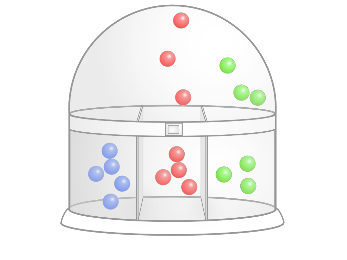
\includegraphics[width=4cm]{draftsinfonijarevisedfinal1-img004.png}&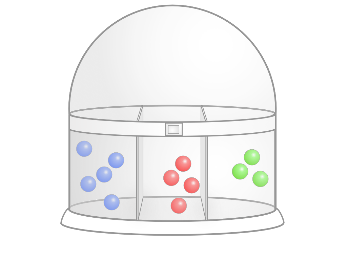
\includegraphics[width=4cm]{draftsinfonijarevisedfinal1-img005.png}&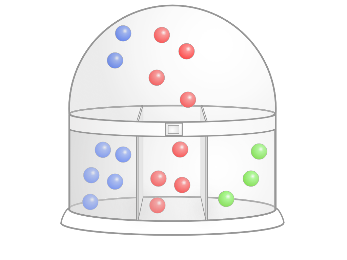
\includegraphics[width=4cm]{draftsinfonijarevisedfinal1-img006.png}\\
\textit{all}-\textsc{early}&\textit{all}-\textsc{late}&\textit{all}-\textsc{garden-path}\\
\end{tabularx}
\caption{The displays for the \textsc{all} condition}
    \label{tom:fig:all}
\end{figure}


%\bigskip

\subsection{Predictions} \label{tom:Predictions}

The visual world studies in \citet{huang2009online, huang2011logic}, \citet{grodner2010some}, and \citet{degen2011making, degen2016availability}
compared the quantifiers \textit{some} and \textit{all} in order to establish whether the processing of the scalar
implicature of \textit{some} is delayed. The literal interpretation of \textit{some}, as in \textit{You got some of the blue
balls}, is that you got at least one
blue ball, so if you got all of them, the sentence is true.\footnote{As observed in \citet{spychalska-msc} in Polish \textit{niektóre} must mean `at least two', because the quantifier occurs only in the plural form.} But in most contexts, we understand this sentence as saying
that we got some blue balls but not all of them. This interpretation is a pragmatic inference: the speaker would have
said ‘You got all of the blue balls’ if we got all of them because that would be a more informative statement.
Quantifiers \textit{all} and \textit{some} form a scale, so when \textit{some} is used instead of the stronger
\textit{all}, the meaning `some-not-all' is inferred -- this inference is called a scalar implicature (\citealt{horn1972, Levinson1983}, a.o.). \citet{huang2009online} found that the `some-not-all' reading was delayed in
comparison with \textit{all}, but \citet{grodner2010some} found no delay and \citet{degen2011making, degen2016availability} hypothesized
that the reason for the delay in \citet{huang2009online} was the availability of other descriptions of the scene:
sentences with number terms in addition to \textit{some }and \textit{all}. \citet{degen2016availability} indeed found that
when no such alternatives were present, the processing of the \textit{some-not-all}-implicature was not delayed
relative to the processing of the meaning of \textit{all}, but it was somewhat delayed when those alternatives were
available. Thus, the processing of pragmatic meaning may be no more costly than the processing of the literal meaning
of a quantifier, depending on the context. In the present experiment, I used the gumball paradigm of \citet{degen2011making, degen2016availability} to investigate the time course of processing of both pragmatic and semantic information. 

Given the findings of \citet{degen2011making, degen2016availability}, the implicature of the Polish `some', \textit{niektóre}, could be
delayed due to the presence of alternative utterances that could describe the same situation. However, \citet{spychalska-msc} argues that the implicature of \textit{niektóre} is stronger than that of English \textit{some}, so if we
find no delay, the current methodology is a useful tool for the investigation of cross-linguistic semantic differences.
To get more specific information about the time course of the processing of \textit{niektóre}, it is compared with the
two majority quantifiers whose literal meaning allows us to make precise predictions for processing, given the findings
in \citet{tomaszewicz2011verification, tomaszewicz2012semantics, tomaszewicz2013linguistic, tomaszewicz2018focus} that each of them drives a distinct verification procedure consistent with its semantics.

The superlative \textit{most} (\textit{most}\textsc{-sup}) in the sentence \textit{You got the most blue balls} (true in the
right top panel of \figref{tom:fig:early}) requires a comparison between the balls in the lower chambers of the machine. In \figref{tom:fig:early},
the machine has dropped down 4 blue, 3 red, 2 green balls. \figref{tom:fig:early} illustrates how the stimulus sentence unfolds: when
hearing the quantifier \textit{najwięcej} (\textit{most}\textsc{-sup}, i.e., ‘the most’), you already know you need
to compare the numbers of the balls and if you had already determined that the blue set is the biggest, you can
anticipate the adjective ‘blue’. The proportional quantifier, \textit{most of}, on the other hand, requires you to
compare the numbers of the blue balls in the lower and the upper chambers. So these two majority quantifiers require
very distinct patterns of eye-movements. The proportion of the looks to the target blue set at the moment of hearing
the quantifier should be lower with \textit{most}\textsc{-sup} because two comparisons are needed (with the
red and the green set) whereas with \textit{most of} just one comparison is necessary (between the lower and upper blue
sets). This predicted contrast between \textit{most of} and \textit{most}\textsc{-sup} allows us to test
whether the looks to the target with \textit{some} will be delayed like with the \textit{most}\textsc{-sup}.
In addition, obtaining this contrast would set up a baseline for further visual world studies on majority quantifiers
cross-linguistically.


% \begin{flushleft}
% \tablefirsthead{}
% \tablehead{}
% \tabletail{}
% \tablelasttail{}
% \begin{supertabular}{m{2.18166in}m{0.41295984in}m{3.6622598in}}
% ~

%  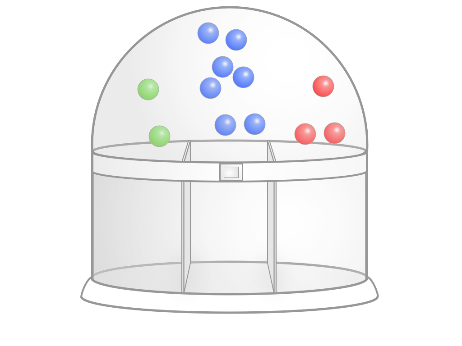
\includegraphics[width=2.0992in,height=1.5752in]{draftsinfonijarevisedfinal1-img007.png}  &
% ~

% ~

% ~

% \textcolor[rgb]{0.5019608,0.5019608,0.5019608}{→}

% ~

% ~
%  &
% ~

%  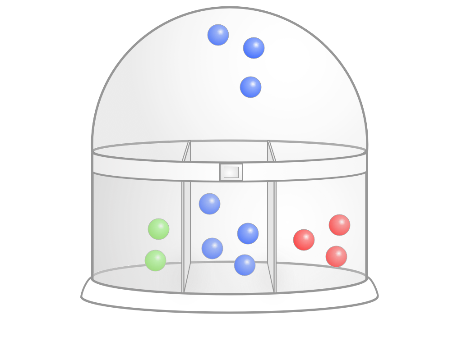
\includegraphics[width=2.0992in,height=1.5752in]{draftsinfonijarevisedfinal1-img008.png} \\
% ~
%  &
% ~
%  &
% Dostałeś najwięcej/większość/niektóre ….\newline
% You.got most\textsc{-sup}/most-of/some ….\\
% ~

%  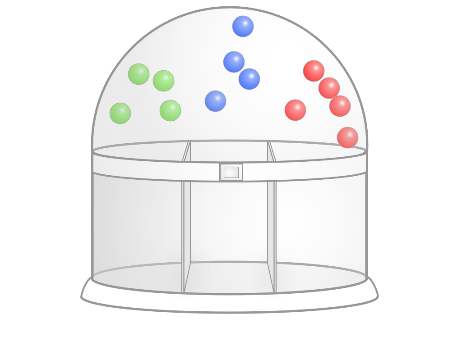
\includegraphics[width=2.0992in,height=1.5752in]{draftsinfonijarevisedfinal1-img009.png}  &
% ~

% ~

% ~

% \textcolor[rgb]{0.5019608,0.5019608,0.5019608}{→}

% ~

% ~
%  &
% ~

%  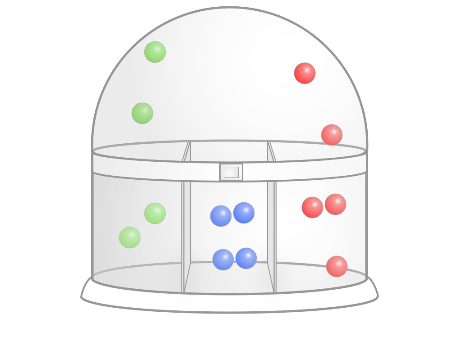
\includegraphics[width=2.0992in,height=1.5752in]{draftsinfonijarevisedfinal1-img010.png} \\
% ~
%  &
% ~
%  &
% Dostałeś wszystkie ….\newline
% You.got all ….\\
% \end{supertabular}
% \end{flushleft}
% \begin{figure}[h]
% \centering
%     \caption{Sample displays in EARLY condition – target: blue.}
%     \label{tom:fig:early}
% \end{figure}

\begin{figure}
    \begin{tikzpicture}
\node(img1) [text width=5.3cm]{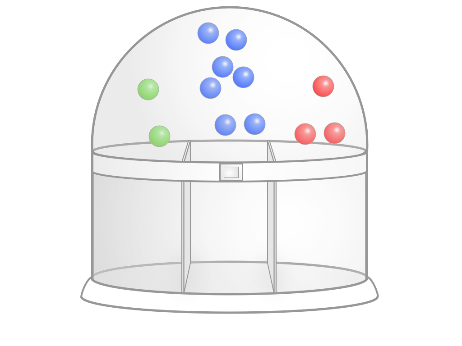
\includegraphics[width=\textwidth]{draftsinfonijarevisedfinal1-img007.png}} ;
\node(img2) [text width=5.3cm,right = 1cm of img1] {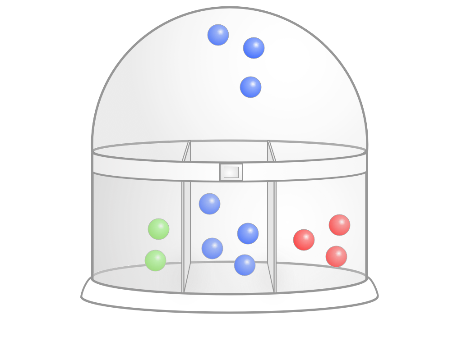
\includegraphics[width=\textwidth]{draftsinfonijarevisedfinal1-img008.png}} ;
\node(text1)[text width=5.3cm,below=1mm of img1] {%\raggedright
};
\node(text2)[text width=5.3cm,below=1mm of img2] {%\raggedright
{\footnotesize Dostałeś najwięcej/większość/niektóre\ldots\newline
`You got most\textsc{-sup}/most-of/some \ldots'}};
\draw[->,thick] (img1) -- (img2);
\node(img3) [text width=5.3cm, below=1.25cm of text1]{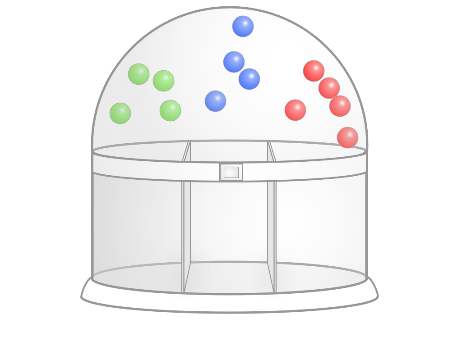
\includegraphics[width=\textwidth]{draftsinfonijarevisedfinal1-img009.png}} ;
\node(img4) [text width=5.3cm,right = 1cm of img3] {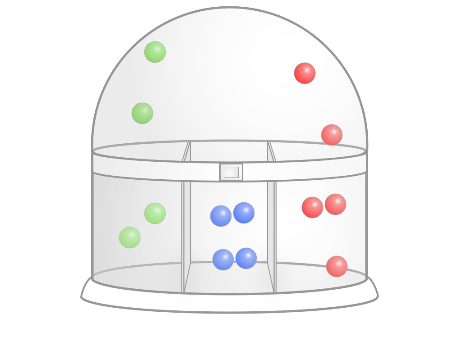
\includegraphics[width=\textwidth]{draftsinfonijarevisedfinal1-img010.png}} ;
\node[text width=5.3cm,below=1mm of img3] {%\raggedright
};
\node[text width=5.3cm,below=1mm of img4] {%\raggedright
{\footnotesize \tabto{1.3cm}Dostałeś wszystkie \ldots\newline
\tabto{1.3cm}`You got all \ldots'}};
\draw[->,thick] (img3) -- (img4);
\end{tikzpicture}
\caption{Sample displays in \textsc{early} condition – target: blue.}
    \label{tom:fig:early}
\end{figure}


%

% \begin{figure} 
%     \begin{tikzpicture}
% \node(img1) [text width=5cm]{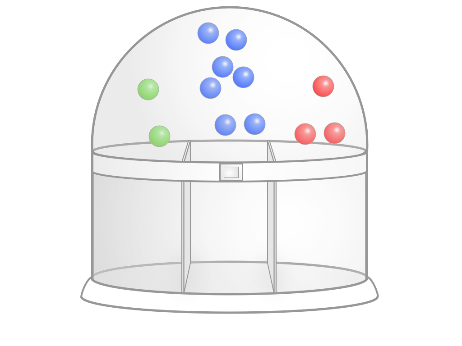
\includegraphics[width=\textwidth]{draftsinfonijarevisedfinal1-img007.png}} ;
% \node(img2) [text width=5cm,right = 1cm of img1] {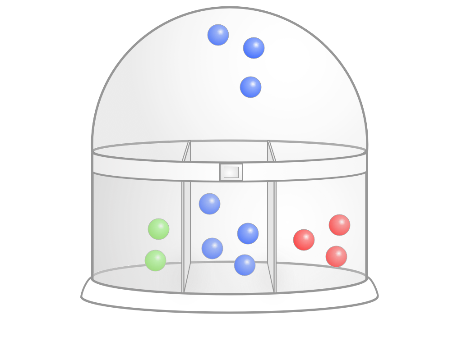
\includegraphics[width=\textwidth]{draftsinfonijarevisedfinal1-img008.png}} ;
% \node(text1)[minimum width=5cm,below=1mm of img1] {%\raggedright
% };
% \node(text2)[minimum width=5cm,below=1mm of img2] {%\raggedright
% \textit{most}\textsc{-sup}/\textit{most of}/\textit{some}};
% \draw[->,thick] (img1) -- (img2);
% \node(img3) [text width=5cm, below=10mm of text1]{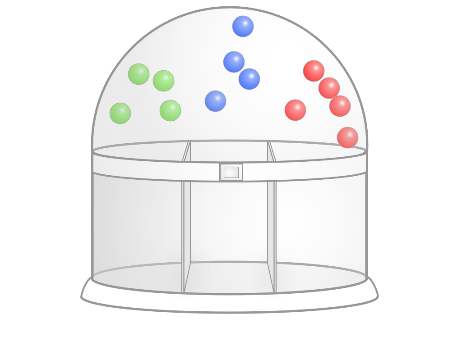
\includegraphics[width=\textwidth]{draftsinfonijarevisedfinal1-img009.png}} ;
% \node(img4) [text width=5cm,right = 1cm of img3] {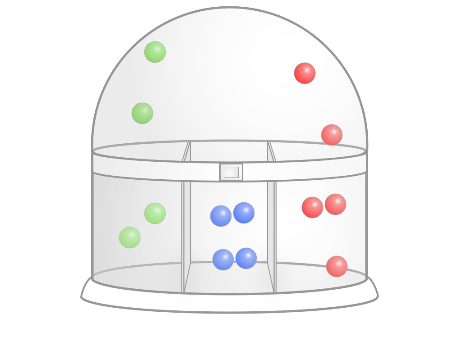
\includegraphics[width=\textwidth]{draftsinfonijarevisedfinal1-img010.png}} ;
% \node[minimum width=5cm,below=1mm of img3] {%\raggedright
% };
% \node[minimum width=5cm,below=1mm of img4] {%\raggedleft
% \textit{all}};
% \draw[->,thick] (img3) -- (img4);
% \end{tikzpicture}
% \caption{Sample displays in \textsc{early} condition – target: blue.}
%     \label{tom:fig:early}
% \end{figure}

%\bigskip

The experiment also includes a comparison with the universal quantifier \textit{all}, but it was not possible to present it together with the same displays as for the three other quantifiers; see the bottom panels of \figref{tom:fig:all}. The displays for \textit{all} contained the same numbers of balls in the lower chambers and the colors were in the same order as in the corresponding displays for the other quantifiers (the exact location of the balls within a chamber was a little different because the displays were generated with a random scatter). The displays for \textit{all} make it very easy to anticipate the color adjective at the point of hearing the quantifier so this condition provides us with a time course for the highest proportion of looks to the target (I already note here that this is not the baseline for statistical comparisons because I want to compare the quantifiers with the same identical displays).

The contrasts described above are predicted for the displays where the quantifier provides a point of disambiguation as to which color is the target set. This is the \textsc{early} condition, i.e., in these displays target identification can happen earlier
than the color adjective is heard. The looks to the target set in the \textsc{early} condition should begin to increase in the quantifier window (as in \citealt{degen2016availability}). In contrast, in the LATE condition, see \figref{tom:fig:late} below, the point of disambiguation is the color adjective.


%\bigskip

% \begin{flushleft}
% \tablefirsthead{}
% \tablehead{}
% \tabletail{}
% \tablelasttail{}
% \begin{supertabular}{m{2.18166in}m{0.41295984in}m{3.6622598in}}
% ~

%  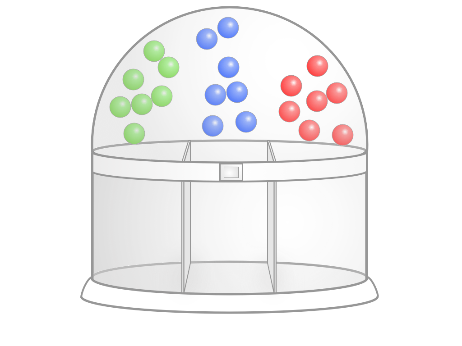
\includegraphics[width=2.0992in,height=1.5752in]{draftsinfonijarevisedfinal1-img011.png}  &
% ~

% ~

% ~

% \textcolor[rgb]{0.5019608,0.5019608,0.5019608}{→}

% ~

% ~

% ~
%  &
% ~

%  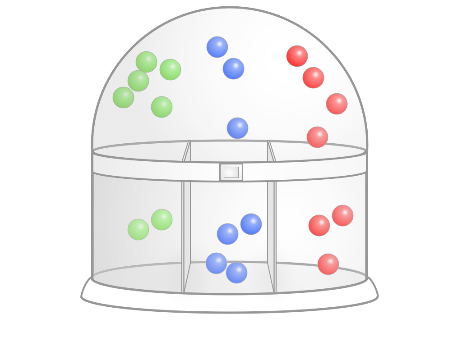
\includegraphics[width=2.0992in,height=1.5752in]{draftsinfonijarevisedfinal1-img012.png} \\
% ~
%  &
% ~
%  &
% Dostałeś większość/najwięcej/niektóre ….\newline
% You-got most-of/most-sup/some ….\\
% ~

%  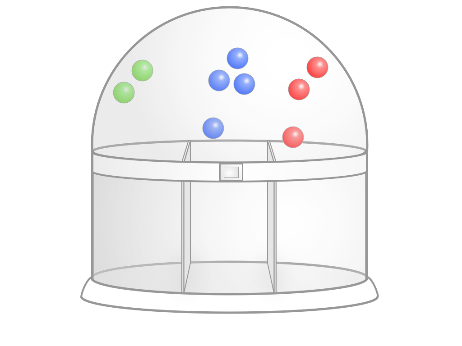
\includegraphics[width=2.0992in,height=1.5752in]{draftsinfonijarevisedfinal1-img013.png}  &
% ~

% ~

% ~

% \textcolor[rgb]{0.5019608,0.5019608,0.5019608}{→}

% ~

% ~
%  &
% ~

%  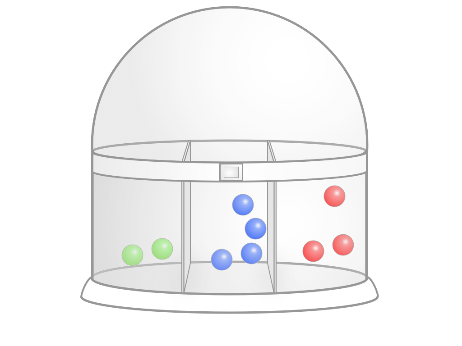
\includegraphics[width=2.0992in,height=1.5752in]{draftsinfonijarevisedfinal1-img014.png} \\
% ~
%  &
% ~
%  &
% Dostałeś wszystkie ….\newline
% You-got all ….\\
% \end{supertabular}
% \end{flushleft}
% \begin{figure}[h]
% \centering
%     \caption{Sample displays in LATE condition – target: blue.}
%     \label{tom:fig:late}
% \end{figure}

\begin{figure} 
    \begin{tikzpicture}
\node(img1) [text width=5.3cm]{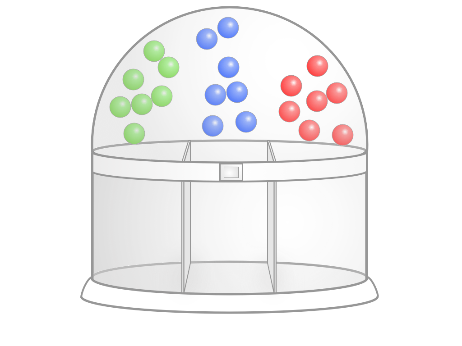
\includegraphics[width=\textwidth]{draftsinfonijarevisedfinal1-img011.png}} ;
\node(img2) [text width=5.3cm,right = 1cm of img1] {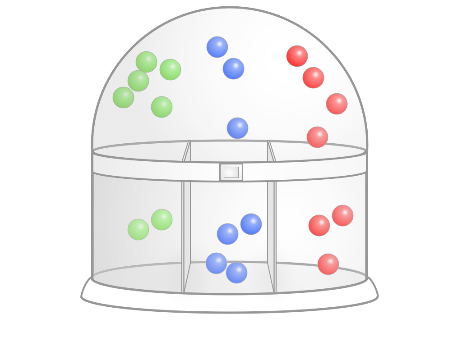
\includegraphics[width=\textwidth]{draftsinfonijarevisedfinal1-img012.png}} ;
\node(text1)[text width=5.3cm,below=1mm of img1] {%\raggedright
};
\node(text2)[text width=5.3cm,below=1mm of img2] {%\raggedright
{\footnotesize Dostałeś większość/najwięcej/niektóre\ldots\newline
`You got most-of/most\textsc{-sup}/some\ldots'}};
\draw[->,thick] (img1) -- (img2);
\node(img3) [text width=5.3cm, below=1.25cm of text1]{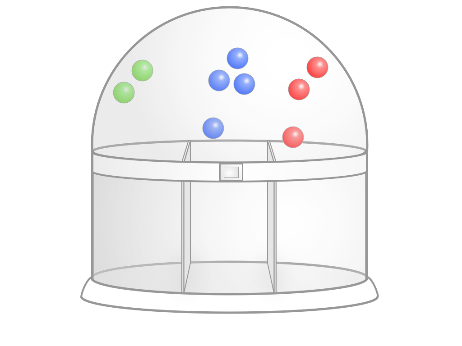
\includegraphics[width=\textwidth]{draftsinfonijarevisedfinal1-img013.png}} ;
\node(img4) [text width=5.3cm,right = 1cm of img3] {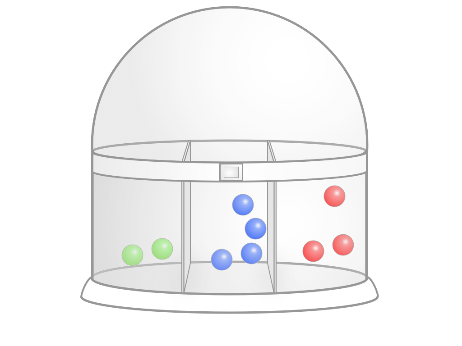
\includegraphics[width=\textwidth]{draftsinfonijarevisedfinal1-img014.png}} ;
\node[text width=5.3cm,below=1mm of img3] {%\raggedright
};
\node[text width=5.3cm,below=1mm of img4] {%\raggedright
{\footnotesize \tabto{1.3cm}Dostałeś wszystkie\ldots\newline
\tabto{1.3cm}`You got all\ldots'}};
\draw[->,thick] (img3) -- (img4);
\end{tikzpicture}
\caption{Sample displays in \textsc{late} condition – target: blue.}
    \label{tom:fig:late}
\end{figure}


%\bigskip

The theoretical predictions outlined above may be affected by possible confounds, because in experiments on visual
identification participants may exhibit different kinds of biases that come, for instance, from the way the visual
system works. One of them is the bias to look more at larger set sizes (also found in the study of \citet{degen2016availability}. This means that already during the preview of the picture, before the sentence is heard, participants will tend
to look at the blue set in the top right panel of Figure \ref{tom:fig:early}. We also know that when precise counting is impossible or simply not needed as in
the current experiment, people use the Approximate Number System (ANS) that generates a representation of magnitude
rather than an exact cardinality, (\citealt{feigenson2004core, dehaene2009origins, dehaene2011number}). It is also known that with a 500\,ms display
ANS automatically enumerates the total set (the superset) and up to two color subsets in parallel, \citep{halberda2006multiple}. Thus, the time course of eye-movements over the three regions of interest is expected to reflect the following
effects in the \textsc{early} condition (the summary is in Table \ref{tom:tab:1:predictions}).

%\bigskip

\subsubsection{Preview and `You got' (\textsc{early})}

During the 500\,ms preview of the display (the right panel of Figures~\ref{tom:fig:machine}--\ref{tom:fig:all}) and during the beginning of the sentence
(\textit{Dostałeś…} `You got…') I expect no differences in the looks to the target for the four quantifiers, except for the
bias to look at the biggest set (the blue target pops out as different than the other two sets, hence it may attract
looks early on).

%\bigskip

\subsubsection{Quantifier (\textsc{early})}

In the \textsc{early} condition, where the quantifier disambiguates which set is the target, in the quantifier window, I expect
fewer looks to the target with \textit{most}\textsc{-sup} than with \textit{most of} and with \textit{all}. The
theoretical prediction explained above is that \textit{most}\textsc{-sup} requires two comparisons (between the blue
and the red set, and between the blue and the green set in the lower chambers), while \textit{most-of} requires one
(between the blue set in the lower chamber and that in the upper chamber). During the preview and the `You got' window
the looks may be attracted to the biggest and partitioned set which is the blue target, therefore in the quantifier
window the looks may already move to the distractors. The quantifier \textit{all} requires no comparisons. This prediction
is summarized as `\textsc{most\textsubscript{sup}} {\textless} \textsc{most-of}, \textsc{all}' in Table \ref{tom:tab:1:predictions} (`fewer looks to the target set in the \textsc{most\textsubscript{sup}} condition than in the \textsc{most-of} and \textsc{all} conditions').

The predictions for \textit{some} in the \textsc{early} condition in the quantifier window depend on which interpretation could
be in the minds of the participants at this point. If the scalar implicature, `some-but-not-all', has already
been processed, the identification of the target should be (almost) just as easy as with \textit{all}: it cannot be the
red nor the green set, and the blue partitioned set has already stood out during preview. Hence, `\textsc{some-not-all}
= \textsc{all}' in Table \ref{tom:tab:1:predictions}. This interpretation would also attract more looks to the blue target than with
\textit{most}\textsc{-sup}, `\textsc{some-not-all} {\textgreater} \textsc{most\textsubscript{sup}}'. If, instead,
participants are first considering the literal meaning of \textit{some}, `some-and-possibly-all', then their
looks will be directed to the green and red color sets as with \textit{most}\textsc{-sup},
`\textsc{some-possibly-all} = \textsc{most\textsubscript{sup}}'.

Finally, there should be more looks to the target in the \textsc{early} condition in the quantifier window with \textit{some} on
the `some-but-not-all' interpretation than with \textit{most of}, `\textsc{some-not-all} {\textgreater}
\textsc{most-of}'. With both quantifiers the looks will be attracted to the partitioned set, the blue target, but with
\textit{most} \textit{of} you need to estimate the numerosities of the two blue subsets and compare them to verify that
the sentence is true.

%\bigskip

\subsubsection{Color\,+\,`balls' (\textsc{early})}

In the \textsc{early} condition, all but one of the effects observed in the quantifier window are predicted to be carried over to
the color window. The exception is the quantifier \textit{most of}, which now may attract a similar proportion of looks
to the target as \textit{some-not-all}, `\textsc{some-not-all} = \textsc{most-of}'. The alternative is that with
\textit{most of} there will still be more looks away from the target, `\textsc{some-not-all} `
\textsc{most-of}', because `\textit{most of the blue balls'} requires more operations for
visual verification than the comparison of the top and bottom blue set as I stated above. \citet{pietroski2009meaning} and \citet{lidz2011interface} propose that sentences with \textit{most of} are verified against visual displays of
multicolored dots not by directly comparing two sets but by a subtraction procedure: you estimate the superset, you
estimate the target set, subtract and compare the result with the target. This procedure involves more steps than
direct comparison of two sets but the reason it is followed is because it is directly specified in the lexical
semantics of the proportional quantifier \textit{most}. \citet{lidz2011interface} argue that sentential meanings are
“individuated more finely than truth conditions” (p. 2) precisely because they interface with perception systems such
as visual cognition. It has been established that numbers can be represented as ``noisy magnitudes'' even for the
purposes of basic arithmetic operations like addition and subtraction (\citealt{feigenson2004core,degen2011making}), so the
subtraction procedure is possible even with a 200\,ms display, but crucially it is less efficient than direct comparison.
This effect was shown in the visual search studies of 
\citet{pietroski2009meaning,lidz2011interface,tomaszewicz2011verification,tomaszewicz2012semantics,tomaszewicz2013linguistic,hunter2017verification, Knowlton2021}, which measured accuracy of Yes-No responses. In the current study I should find
evidence that participants follow the subtraction procedure, as specified in (\ref{tom:ex:subtraction}), in contrast to direct selection of
the two sets as in (\ref{tom:ex:selection}), if we find fewer looks to the target in the color window than with \textsc{some-not-all}
because of continuing looks to the top blue set in order to establish the total set. Perhaps, the proportion of looks
to the target will even be as low as with \textit{most}\textsc{-sup}\textit{ }(`\textsc{some-not-all} = \textsc{most-of}?\slash \textsc{some-not-all} {\textgreater} \textsc{most-of}\slash \textsc{most-of} = \textsc{most\textsubscript{sup}}?' in Table \ref{tom:tab:1:predictions}). Such a result in the color window in the \textsc{early} condition would provide
support for a higher number of processing steps involved in (\ref{tom:ex:subtraction}) as opposed to (\ref{tom:ex:selection}). 

%\bigskip

\ea \textsc{subtraction} procedure for the verification of the sentence `You got \textit{most of }the blue balls':

\#[\textsc{blue(x)} \& \textsc{below(x)}] {\textgreater} \#[\textsc{blue(x)} \& \textsc{above(x)} \& \textsc{below(x)}] – [\textsc{blue(x)} \& \textsc{above(x)}]\\
\label{tom:ex:subtraction}

%\bigskip

\ex \textsc{selection} procedure for the verification of the sentence `You got \textit{most of }the blue balls':

\#[\textsc{blue(x)} \& \textsc{below(x)}] {\textgreater} \#[\textsc{blue(x)} \& \textsc{above(x)}]
\label{tom:ex:selection}
\z
The differences expected to occur in the \textsc{late} condition are presented in the following subsections.

% \begin{table}
% \caption{Predictions}
% \label{tom:tab:1:predictions}
% % \begin{tabularx}{.8\textwidth}{cccc} 
%     \begin{tabular}{cccc} 
%     \lsptoprule
%   \multicolumn{4}{l}{\textbf{EARLY}}\\
%   \midrule
%         Preview & `You got' & \thead{Quantifier \\ \textit{point of disambiguation} } & Color+`balls'\\ 
%   \midrule
%   \multicolumn{2}{c}{No differences / Big set bias?}  &
%   \thead{\textsc{most\textsubscript{sup}} {\textless} \textsc{most-of} \& \textsc{all} \\ \textsc{some-not-all} = \textsc{all} \\ \textsc{some-not-all} {\textgreater} \textsc{most\textsubscript{sup}} \\ \textsc{some-possibly-all} = \textsc{most\textsubscript{sup}} \\ \textsc{some-not-all} {\textgreater} \textsc{most-of}} &
  
%   \thead{\textsc{\mygraycolor{Most}}\mygraycolor{\textsubscript{SUP}}\mygraycolor{{\textless}}\textsc{\mygraycolor{Most-Of}}\mygraycolor{\&}\textsc{\mygraycolor{All}}\\
%   \textsc{\mygraycolor{Some}}\mygraycolor{{}-not all=}\textsc{\mygraycolor{All}}\\
%   \textsc{\mygraycolor{Some}}\mygraycolor{{}-not all{\textgreater}}\textsc{\mygraycolor{Most}}\mygraycolor{\textsubscript{SUP}}\\
%   \textsc{\mygraycolor{Some-possibly-all}}\mygraycolor{=}\textsc{\mygraycolor{Most}}\mygraycolor{\textsubscript{SUP}}\\
%   \textsc{some-not-all} = \textsc{most-of}? /\\ \textsc{some-not-all} {\textgreater} \textsc{most-of} /\\ \textsc{most-of} =\textsc{most\textsubscript{sup}}?}\\
  
%   \midrule
  
%   \multicolumn{4}{l}{\textbf{LATE}}\\
%   \midrule
%         Preview & `You got' & Quantifier & \thead{Color+`balls' \\ \textit{point of disambiguation} }\\ 
%   \midrule
%   \multicolumn{2}{c}{No differences}  &
%   \thead{\textsc{most\textsubscript{sup}} {\textgreater} \textsc{all}, \textsc{most-of}, \textsc{some} \\
%   \textsc{some-not-all} {\textgreater} \textsc{most-of}\\
%   \textsc{some-not-all} {\textless} \textsc{all}} &
   
%   \thead{\textsc{most\textsubscript{sup}} {\textless} \textsc{all}, \textsc{most-of}, \textsc{some}\\
%   \textsc{\mygraycolor{Some-not-all}}\mygraycolor{ {\textgreater}}\textsc{\mygraycolor{Most-Of}}\\
%   \textsc{\mygraycolor{Some-not-all}}\mygraycolor{ {\textless}}\textsc{\mygraycolor{All}}}\\
%   \lspbottomrule
% % \end{tabularx}
%     \end{tabular}
% \end{table}

\begin{table}[h]\small
\caption{Predictions\label{tom:tab:1:predictions}. (†) marks the \textit{point of disambiguation}.}
\begin{subtable}{\textwidth}
\caption{\textsc{early}}
    \begin{tabularx}{\textwidth}{llXX}
    \lsptoprule
        Preview & `You got' & Quantifier (†)& Color\,+\,`balls'\\\midrule
  \multicolumn{2}{l}{No differences/}  &{
  \textsc{most\textsubscript{sup}} {\textless} \textsc{most-of} \& \textsc{all}}&{\mygraycolor{\textsc{most\textsubscript{sup} {\textless} most-of} \& \textsc{all}}}\\
  \multicolumn{2}{l}{Big set bias?}&{\textsc{some-not-all} = \textsc{all}}&{\textsc{\mygraycolor{some-not-all = all}}}\\
  &&{\textsc{some-not-all} {\textgreater} \textsc{most\textsubscript{sup}}}&{\textsc{\mygraycolor{some-not-all {\textgreater} most\textsubscript{sup}}}}\\
  &&{\textsc{some-possibly-all} = \textsc{most\textsubscript{sup}}}&{\textsc{\mygraycolor{some-possibly-all = most\textsubscript{sup}}}}\\
  &&{\textsc{some-not-all} {\textgreater} \textsc{most-of}}&{\textsc{some-not-all} = \textsc{most-of}? /}\\
  &&&{\textsc{some-not-all} {\textgreater} \textsc{most-of} /}\\
  &&&{\textsc{most-of} = \textsc{most\textsubscript{sup}}?}\\
  \lspbottomrule
  \end{tabularx}
\end{subtable}\medskip\\
\begin{subtable}{\textwidth}
\caption{\textsc{late}}
    \begin{tabularx}{\textwidth}{llXX}
    \lsptoprule
        Preview & `You got' & Quantifier &Color\,+\,`balls' (†)\\\midrule
  \multicolumn{2}{l}{No differences}  &
   {\textsc{most\textsubscript{sup}} {\textgreater} \textsc{all}/\textsc{most-of}/\textsc{some}}&{\textsc{most\textsubscript{sup}} {\textless} \textsc{all}/\textsc{most-of}/\textsc{some}}\\
   &&{\textsc{some-not-all} {\textgreater} \textsc{most-of}}&{\textsc{\mygraycolor{some-not-all {\textgreater} most-of}}}\\
   &&{\textsc{some-not-all} {\textless} \textsc{all}}&{\textsc{\mygraycolor{some-not-all {\textless} all}}}\\
  \lspbottomrule
    \end{tabularx}
    \end{subtable}
\end{table}


\subsubsection{Preview and `You got' (\textsc{late})}

I expect no differences. As can be seen in \figref{tom:fig:late}, bottom-right panel, the target set cannot be identified during the
preview by the big set bias (the blue bottom set is not the only large set).
\bigskip

\subsubsection{Quantifier (\textsc{late})}

In the \textsc{late} condition, the target set can only be reliably disambiguated upon hearing the color adjective, that is, in
the last time window of interest. However, I do expect differences in the quantifier window already.

Because the target set cannot be biased during the preview, upon hearing the quantifier \textit{most}\textsc{-sup}, the
looks could be immediately directed to the largest of the bottom sets, the blue target, while with \textit{most of} and
\textit{some} the looks will also be directed to the upper sets and with \textit{all} to the other bottom sets. Thus,
the prediction is `\textsc{most\textsubscript{sup}} {\textgreater} \textsc{all}, \textsc{most-of}, \textsc{some}' in
Table \ref{tom:tab:1:predictions}. Alternatively, the identification of the largest set with \textit{most}\textsc{-sup} is delayed until the
color window, but given the big set bias, I find this option unlikely.

I also expect more looks to the target with \textit{some-not-all} than \textit{most of} because \textit{most of}
requires the estimation of the numerosity of the bottom blue set relative to the top set (in one of the two ways in (\ref{tom:ex:subtraction}--\ref{tom:ex:selection}) discussed above). Additionally, there should be fewer looks to the target with \textit{some-not-all} than with
\textit{all} because the set for the latter is unpartitioned. These two effects should persist in the color window.

In the \textsc{late} condition, the \textit{some-possibly-all} interpretation is not tested because all sets are partitioned.
%\bigskip

\subsubsection{Color\,+\,`balls' (\textsc{late})}

At the point of hearing the color adjective in the \textsc{late} condition, the proportion of looks to the target with
\textit{most}\textsc{-sup} should be lower than with other quantifiers because now the looks are attracted to the
other two color sets in order to make the comparisons to confirm that indeed the blue set is the largest,
`\textsc{most\textsubscript{sup}} {\textless} \textsc{all}, \textsc{most-of}, \textsc{some}'. Could it be that once the
largest set is identified already in the quantifier window, participants stop making the comparisons upon hearing `blue' because it matches the already identified target? I do not think so, simply because the `identification of the target' as early as the quantifier happens unconsciously, and only when the color is heard are the participants aware of the semantics of the full sentence, thus I expect the processing to keep going and to follow the semantics of the
superlative sentence: `There are more blue balls than the balls in any other color'. Accordingly, I expect that in the color window, comparisons with other colors will take place.
%\bigskip

Of all of the above, the predictions of main theoretical interest are the following: 

\begin{enumerate}[label=(\roman*)]
\item In the \textsc{early} condition, at the quantifier (which disambiguates the target set) there will be fewer looks to the
target with \textsc{most\textsubscript{sup}} than \textsc{most-of} and \textsc{all} because the superlative semantics
requires comparisons with other color sets, \textsc{most\textsubscript{sup}} {\textless} \textsc{most-of} \&
\textsc{all}. The looks to the target with \textsc{most\textsubscript{sup}} can serve as the baseline for establishing if the implicature of
\textit{niektóre} `some' is processed early: \textsc{some-not-all} {\textgreater} \textsc{most\textsubscript{sup}} vs.
\textsc{some-possibly-all} = \textsc{most\textsubscript{sup}}.

\item In the \textsc{early} condition, in the last region (Color\,+\,`balls'), with \textsc{most-of} the looks will either stay on the target as with \textsc{some} (if participants follow the direct Selection procedure in (\ref{tom:ex:selection})), \textsc{some-not-all} = \textsc{most-of}, or there will be fewer looks to the target (if participants need to establish the total set of blue balls for the Subtraction procedure in (\ref{tom:ex:subtraction})), \textsc{some-not-all} {\textgreater} \textsc{most-of}, \textsc{most-of} = \textsc{most\textsubscript{sup}}.

\item In the \textsc{late} condition, at the quantifier, there should be more looks to the target with
\textsc{most\textsubscript{sup}} than with the other quantifiers, reflecting the immediate processing of the superlative
semantics, \textsc{most\textsubscript{sup}} {\textgreater} \textsc{all}, \textsc{most-of}, \textsc{some}.

\item In the \textsc{late} condition, at the disambiguation point (Color\,+\,`balls'), the looks to the target with \textsc{most\textsubscript{sup}} should decline, \textsc{most\textsubscript{sup}} {\textless} all, \textsc{most-of}, \textsc{some}, because the semantics requires comparisons with other color sets.
\end{enumerate}


%\bigskip

\subsection{Results: Behavioral} 

The mean accuracy on the test conditions (i.e, \textsc{early} and \textsc{late} that required a Yes response) was 95\%. Of the 35
participants, 30 got 97--100\% correct and 3 got less than 70\% correct (54\%, 58\%, 65\%). I kept all of the responses
because I did not aggregate the data for statistical analyses and I used the eye-movement data only from the correct
trials. I removed the extremely long outlier reaction times (three standard deviations above the mean); those
constituted 1.3\% of the Yes and No data and were equally found in all conditions and regions of interest. The accuracy
of the responses and reaction times (RTs) are plotted in \figref{tom:fig:plots}.

\begin{figure} 
    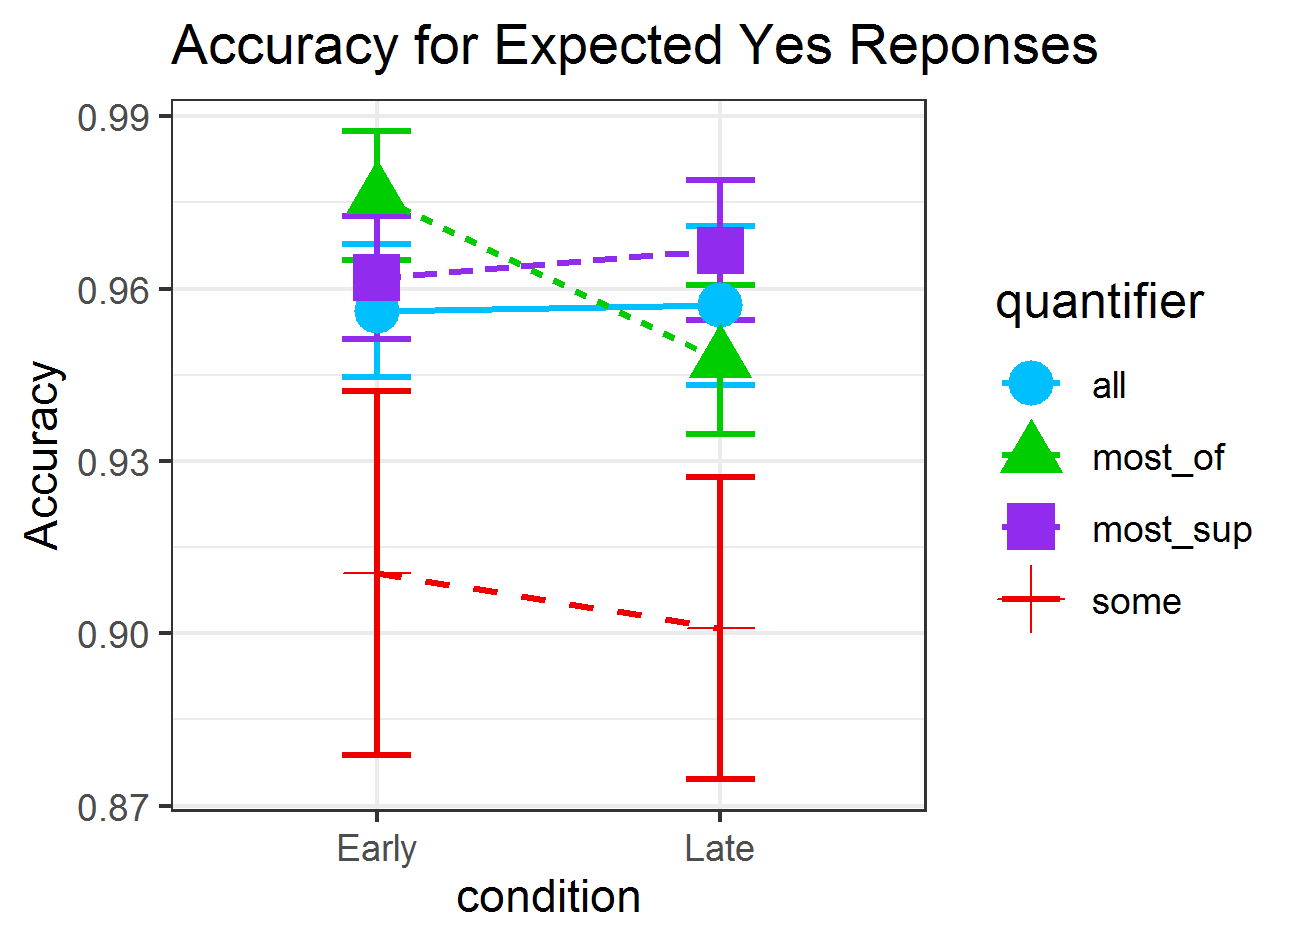
\includegraphics[width=.475\textwidth]{draftsinfonijarevisedfinal1-img015.png}\hfill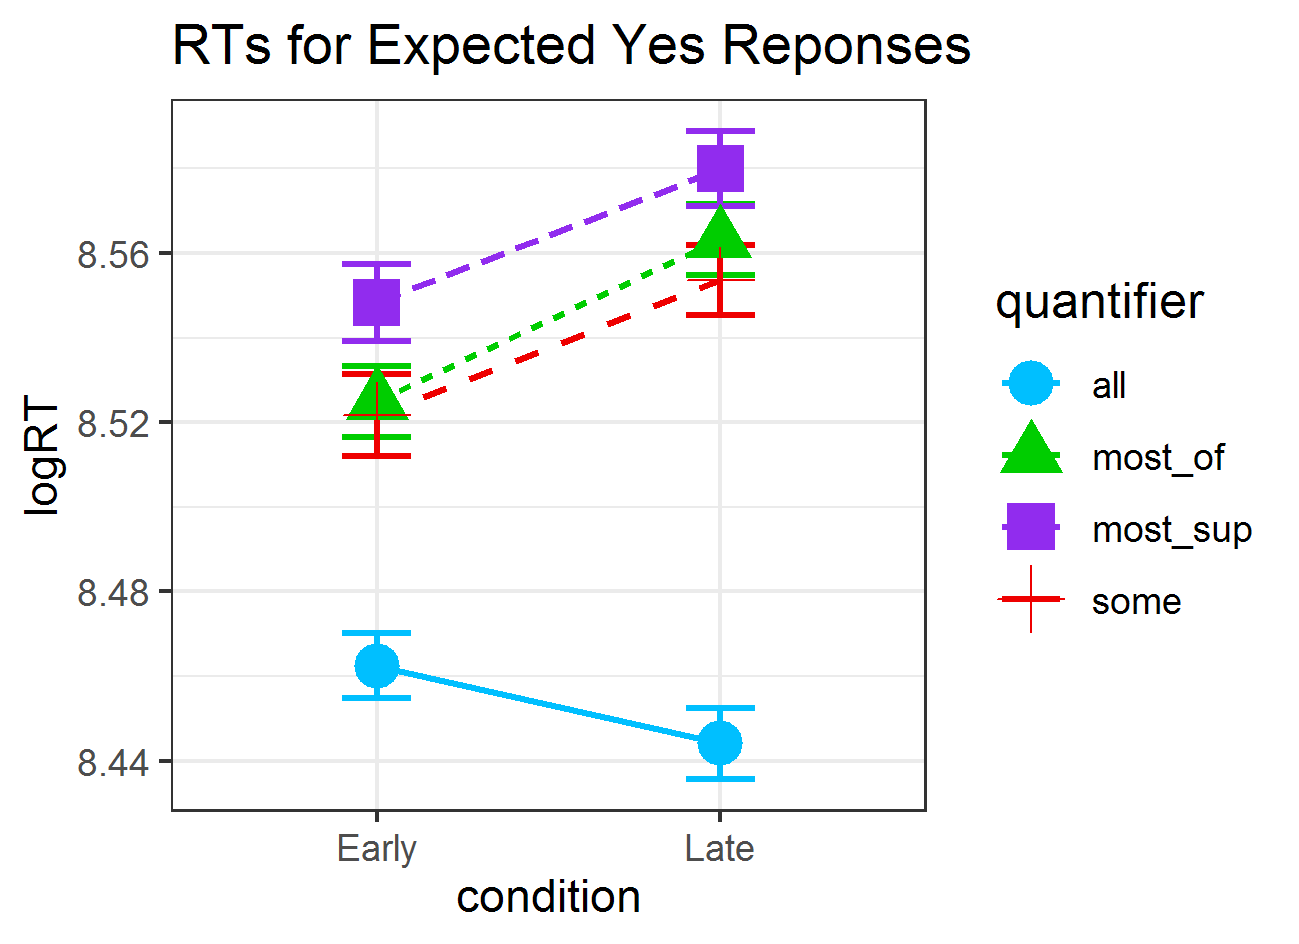
\includegraphics[width=.475\textwidth]{draftsinfonijarevisedfinal1-img016.png}
\caption{Accuracy and log-transformed reaction times (error bars represent standard errors)\label{tom:fig:plots}}
\end{figure}


I fitted a mixed-effects regression model of the log-transformed RTs and a mixed effects logistic regression model of
the (binary) yes/no variable in R version 3.6.2 \citep{rcore}  using the lme4 package version 1.1-21 \citet{lme4}. The \textit{p}{}-values were obtained using model comparison and the Satterthwaite approximation implemented in
the lmerTest package \citep{kuznetsova2017lmertest}. 

For the accuracy data, there is a significant main effect of quantifier ($\chi ^2=13.72, \text{df}=3,
p=0.003$). With ANOVA-style contrast coding, there are no differences in pairwise comparisons between the
conditions. There are also no differences in pairwise comparisons when \textsc{all} is the baseline; with \textsc{some} as the baseline only \textsc{most-of} is significantly different, $\beta =2.066, \text{SE}=0.758, t=2.742, p=0.026$ (including the Bonferroni correction for multiple comparisons). Summing up, the accuracy across the conditions ranged from 87\% to 99\%, and participants were significantly less accurate in the \textsc{some} condition in comparison to the \textsc{most-of} condition. We do not see such a difference in reaction times (right panel in \figref{tom:fig:plots}): \textsc{some} is not slower than the other conditions, which means that
this condition was not harder, but either that people were fast and made mistakes (which is unlikely given that
\textsc{most-of} and \textsc{most\textsubscript{sup}} had similar RTs) or rather that they believed ‘No, I did
not get \textit{some} of the balls in color x, I got \textit{most} of them.’

The plot of the RTs in \figref{tom:fig:plots} shows significant effects of the \textsc{early}/\textsc{late} condition ($\chi^2=9.39,
\text{df}=1, p=0.002$) and Quantifier ($\chi^2=72.91, \text{df}=3, p<0.0001$) and their
interaction ($\chi^2=11.62, \text{df}=3, p=0.009$). Pairwise-comparisons with
\textsc{most\textsubscript{sup}} as the baseline confirm what we see in the plot: that only the \textsc{all}
condition is significantly faster ($\beta =-0.085, \text{SE}=0.014, t=-6.085,\allowbreak p<0.0001$). This is
expected given that as discussed in \sectref{tom:Methods}, \textsc{all} had the easiest screens (since the accuracy with
\textsc{all}, \textsc{most\textsubscript{sup}} and \textsc{most-of} was very high, we do not see differences due to the difficulty of the screens).

Note that while the semantics of \textsc{most\textsubscript{sup}} requires comparisons with the two other color sets in the bottom chamber, we see that these comparison procedures have no effect on the accuracy nor on the reaction times. This is compatible with the predictions (as summarized in Table \ref{tom:tab:1:predictions}) where on the \textsc{early} condition, looks to the
target with \textsc{most\textsubscript{sup}} could benefit from the big set bias in the first two time windows
with the rest of the time spent on looking at the other colors; on the \textsc{late} condition in the quantifier window there
should be more looks to the target and then fewer in the color window than with the other quantifiers. In the next
section we will see that the predicted differences are in fact reflected in the eye movements.


%\bigskip

\subsection{Results: Eye-movements} 

The pre-processing of the eye-movement data and plotting was carried out using the VWPre package (version 1.2.2,
\citealt{Porretta}). The first line in Figures \ref{tom:tab:2:early}--\ref{tom:tab:3:late} shows the plots of the proportion of looks to the target for the \textsc{early} and \textsc{late}
conditions. The black lines mark the time windows in the audio stimulus adjusted by 200\,ms (i.e., 200\,ms post the
actual onset).\footnote{\textrm{200\,ms was chosen following \citet{degen2016availability} because the earliest language
mediated fixations are at 200--250\,ms after the relevant acoustic landmark that could establish a point of
disambiguation \citep{salverda2014immediate}} The proportion of looks for each interest area has been
converted to empirical logits because proportions are inherently bound between 0 and 1 but logits provide a
transformation resulting in an unbounded measure suitable for use in the statistical tests \citep{barr2008analyzing}.}

I fitted generalized additive mixed models (GAMMs) using the packages mgcv (version 1.8-31; \citealt{wood2017package,wood2017generalized}) and
itsadug (version 2.3; \citealt{itsadug}) to the eye data because a regression line is unable to capture the
nonlinear nature of the time course data as in Figures \ref{tom:tab:2:early}--\ref{tom:tab:3:late}. GAMM is a nonlinear regression analysis which in addition to
linear effects includes smooth terms as well as random smooths to capture the random effects. Model comparisons involve
the full model, with all terms and interactions, and a nested model that excludes the main term and the smooth term
corresponding to the predictor and the interactions with these terms (\citealt{winter2016analyze,soskuthy2017generalised,wood2017generalized}). Because in this experiment the predictions are only about the parametric terms (the proportion of looks to the
target within a given time window) and not about the differences between the shapes of the curves, significance testing
is based on the \textit{t}{}-values and I only report those.

The third line in Figures \ref{tom:tab:2:early}--\ref{tom:tab:3:late} shows the model predictions for each of the time windows without random smooths, Preview
($-500$--0\,ms), \textit{Dostałeś} `You got' (0--1030\,ms), the quantifier (1030--2122\,ms),
\textit{niebieskich\slash zielonych\slash czerwonych kulek} `blue\slash green\slash red balls' (2122--3682\,ms). The fourth line shows the model
predictions including the random smooths that capture the random effects of Subject, Item and Trial. The fifth line
summarizes the statistical findings showing which of the contrasts were significant -- the unpredicted significant
effects are highlighted in grey. The non-highlighted findings match the predictions summarized in Table \ref{tom:tab:1:predictions}.

In the \textsc{early} condition, Figures \ref{tom:tab:2:early}, there is a main effect of Quantifier in each time window (Preview: $\chi^2=10.96, \text{df}=9,
p=0.009$; `You got': $\chi^2=105.5, \text{df}=9,\allowbreak p<0.0001$; the quantifier: $\chi^2=55.8, 
\text{df}=9,
p<0.0001$; the color window: $\chi^2=140.35, \text{df}=9, p<0.0001$). Pairwise
comparisons reveal the following differences ($p$-values include the Bonferroni correction for multiple comparisons):

In the Preview window, there are more looks to the target with \textsc{most\textsubscript{sup}} than with
\textsc{most-of} ($\beta =-0.388, \text{SE}=0.119, t=-3.268, p=0.004$) and with \textsc{some} than
\textsc{most-of} ($\beta =-0.389, \text{SE}=0.107, t=-3.617, p=0.001$).

In the `You got' window, the proportion of looks to the target is higher with \textsc{most\textsubscript{sup}} than with
\textsc{some} ($\beta =-0.653, \text{SE}=0.102, t=-6.382, p<0.0001$) and than with
\textsc{most-of} ($\beta =-1.259, SE 0.111, t=-11.377, p<0.0001$), as well as with
\textsc{some} in comparison with \textsc{most-of} ($\beta =-0.604, \text{SE}=0.101, t=-6.011,\allowbreak
p<0.0001$).

In the quantifier window, the trend is reversed and there are fewer looks to the target with
\textsc{most\textsubscript{sup}} than with \textsc{some} ($\beta =0.637, \text{SE}=0.115, t=5.528,
p<0.0001$) and with \textsc{most-of} ($\beta =0.866, \text{SE}=0.123, t=7.02,
p<0.0001$).

In the color adjective plus noun `balls' window, there are still fewer looks to the target with
\textsc{most\textsubscript{sup}} than with \textsc{some} ($\beta =0.574, \text{SE}=0.106, t=5.436,\allowbreak
p<0.0001$). But now there is no difference between \textsc{most\textsubscript{sup}} and
\textsc{most-of}. There are now fewer looks to the target with \textsc{most\textsubscript{sup}} than with \textsc{all}
($\beta =1.761,\allowbreak \text{SE}=0.166, t=10.6, p<0.0001$). Also \textsc{some} has fewer looks to the
target than \textsc{all} ($\beta =0.95, \text{SE}=0.172, t=5.533, p<0.0001$), but it has more
looks to the target than \textsc{most-of} ($\beta =-0.41, \text{SE}=0.102, t=-4.003, p=0.0002$).

% \begin{figure}[h]
%     \centering
%     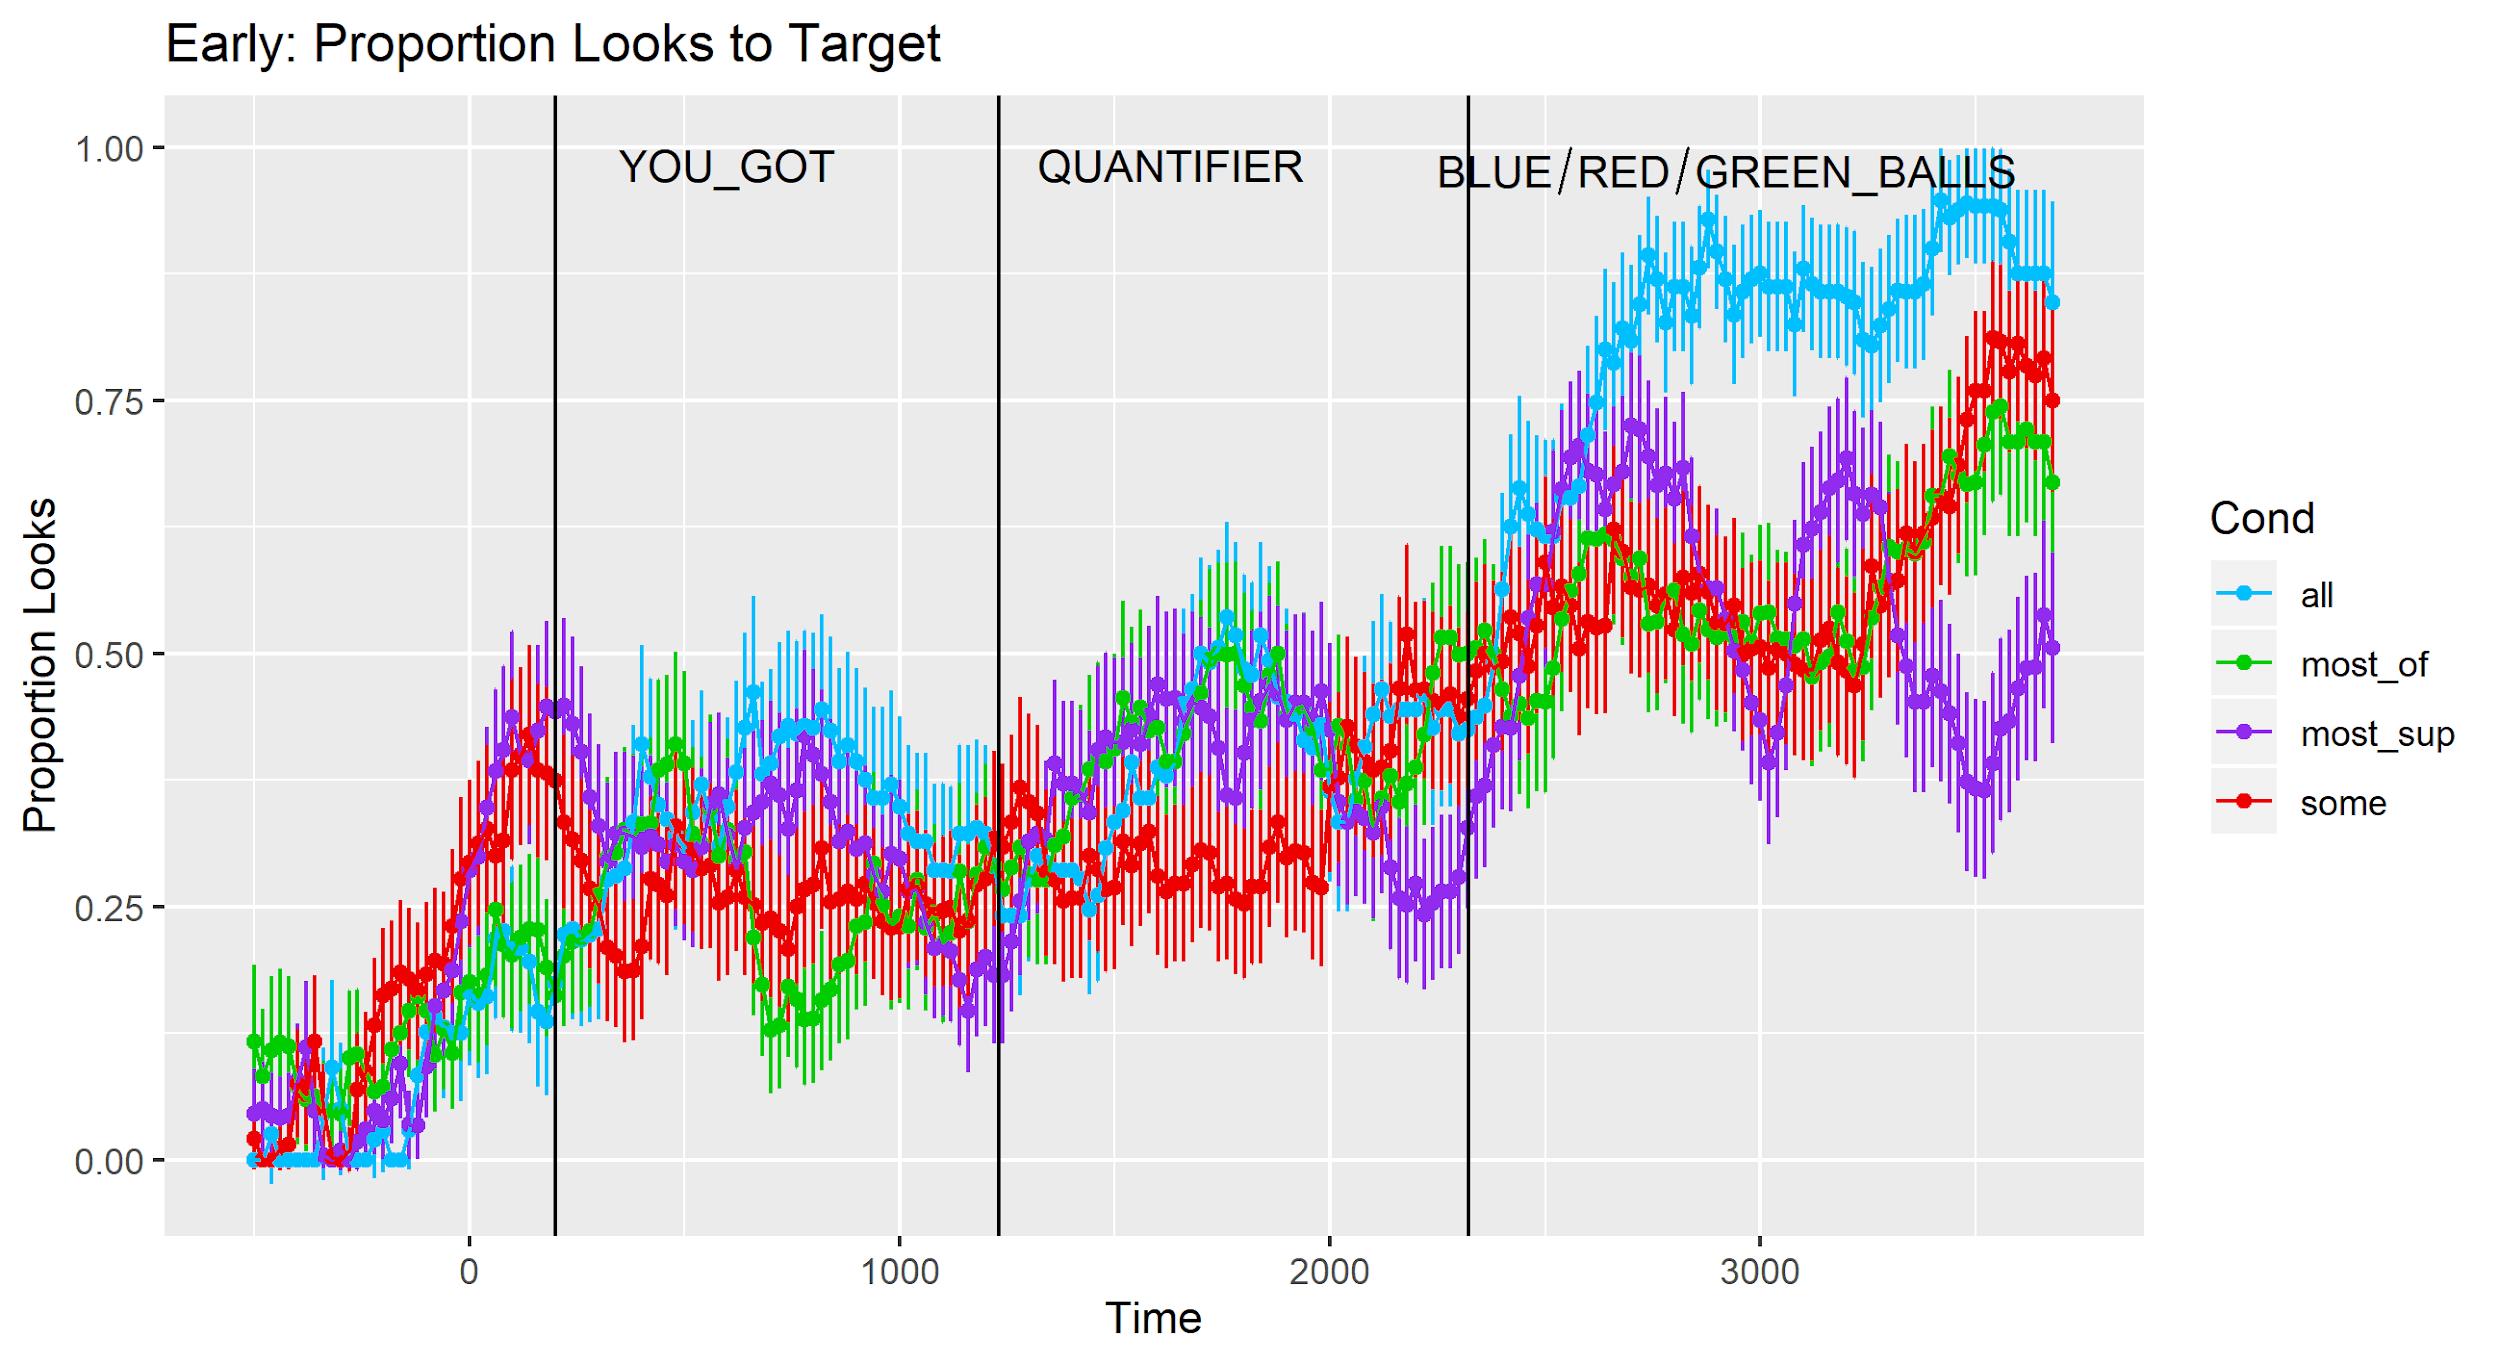
\includegraphics[width=\textwidth]{draftsinfonijarevisedfinal1-img017.png}
%     \caption{ADD CAPTION}
%     \label{tom:fig:result-early}
% \end{figure}


\begin{figure}[p]\small
\centering
\caption{Results: \textsc{early} condition. (†) marks \textit{disambiguation}.}
\label{tom:tab:2:early}
% 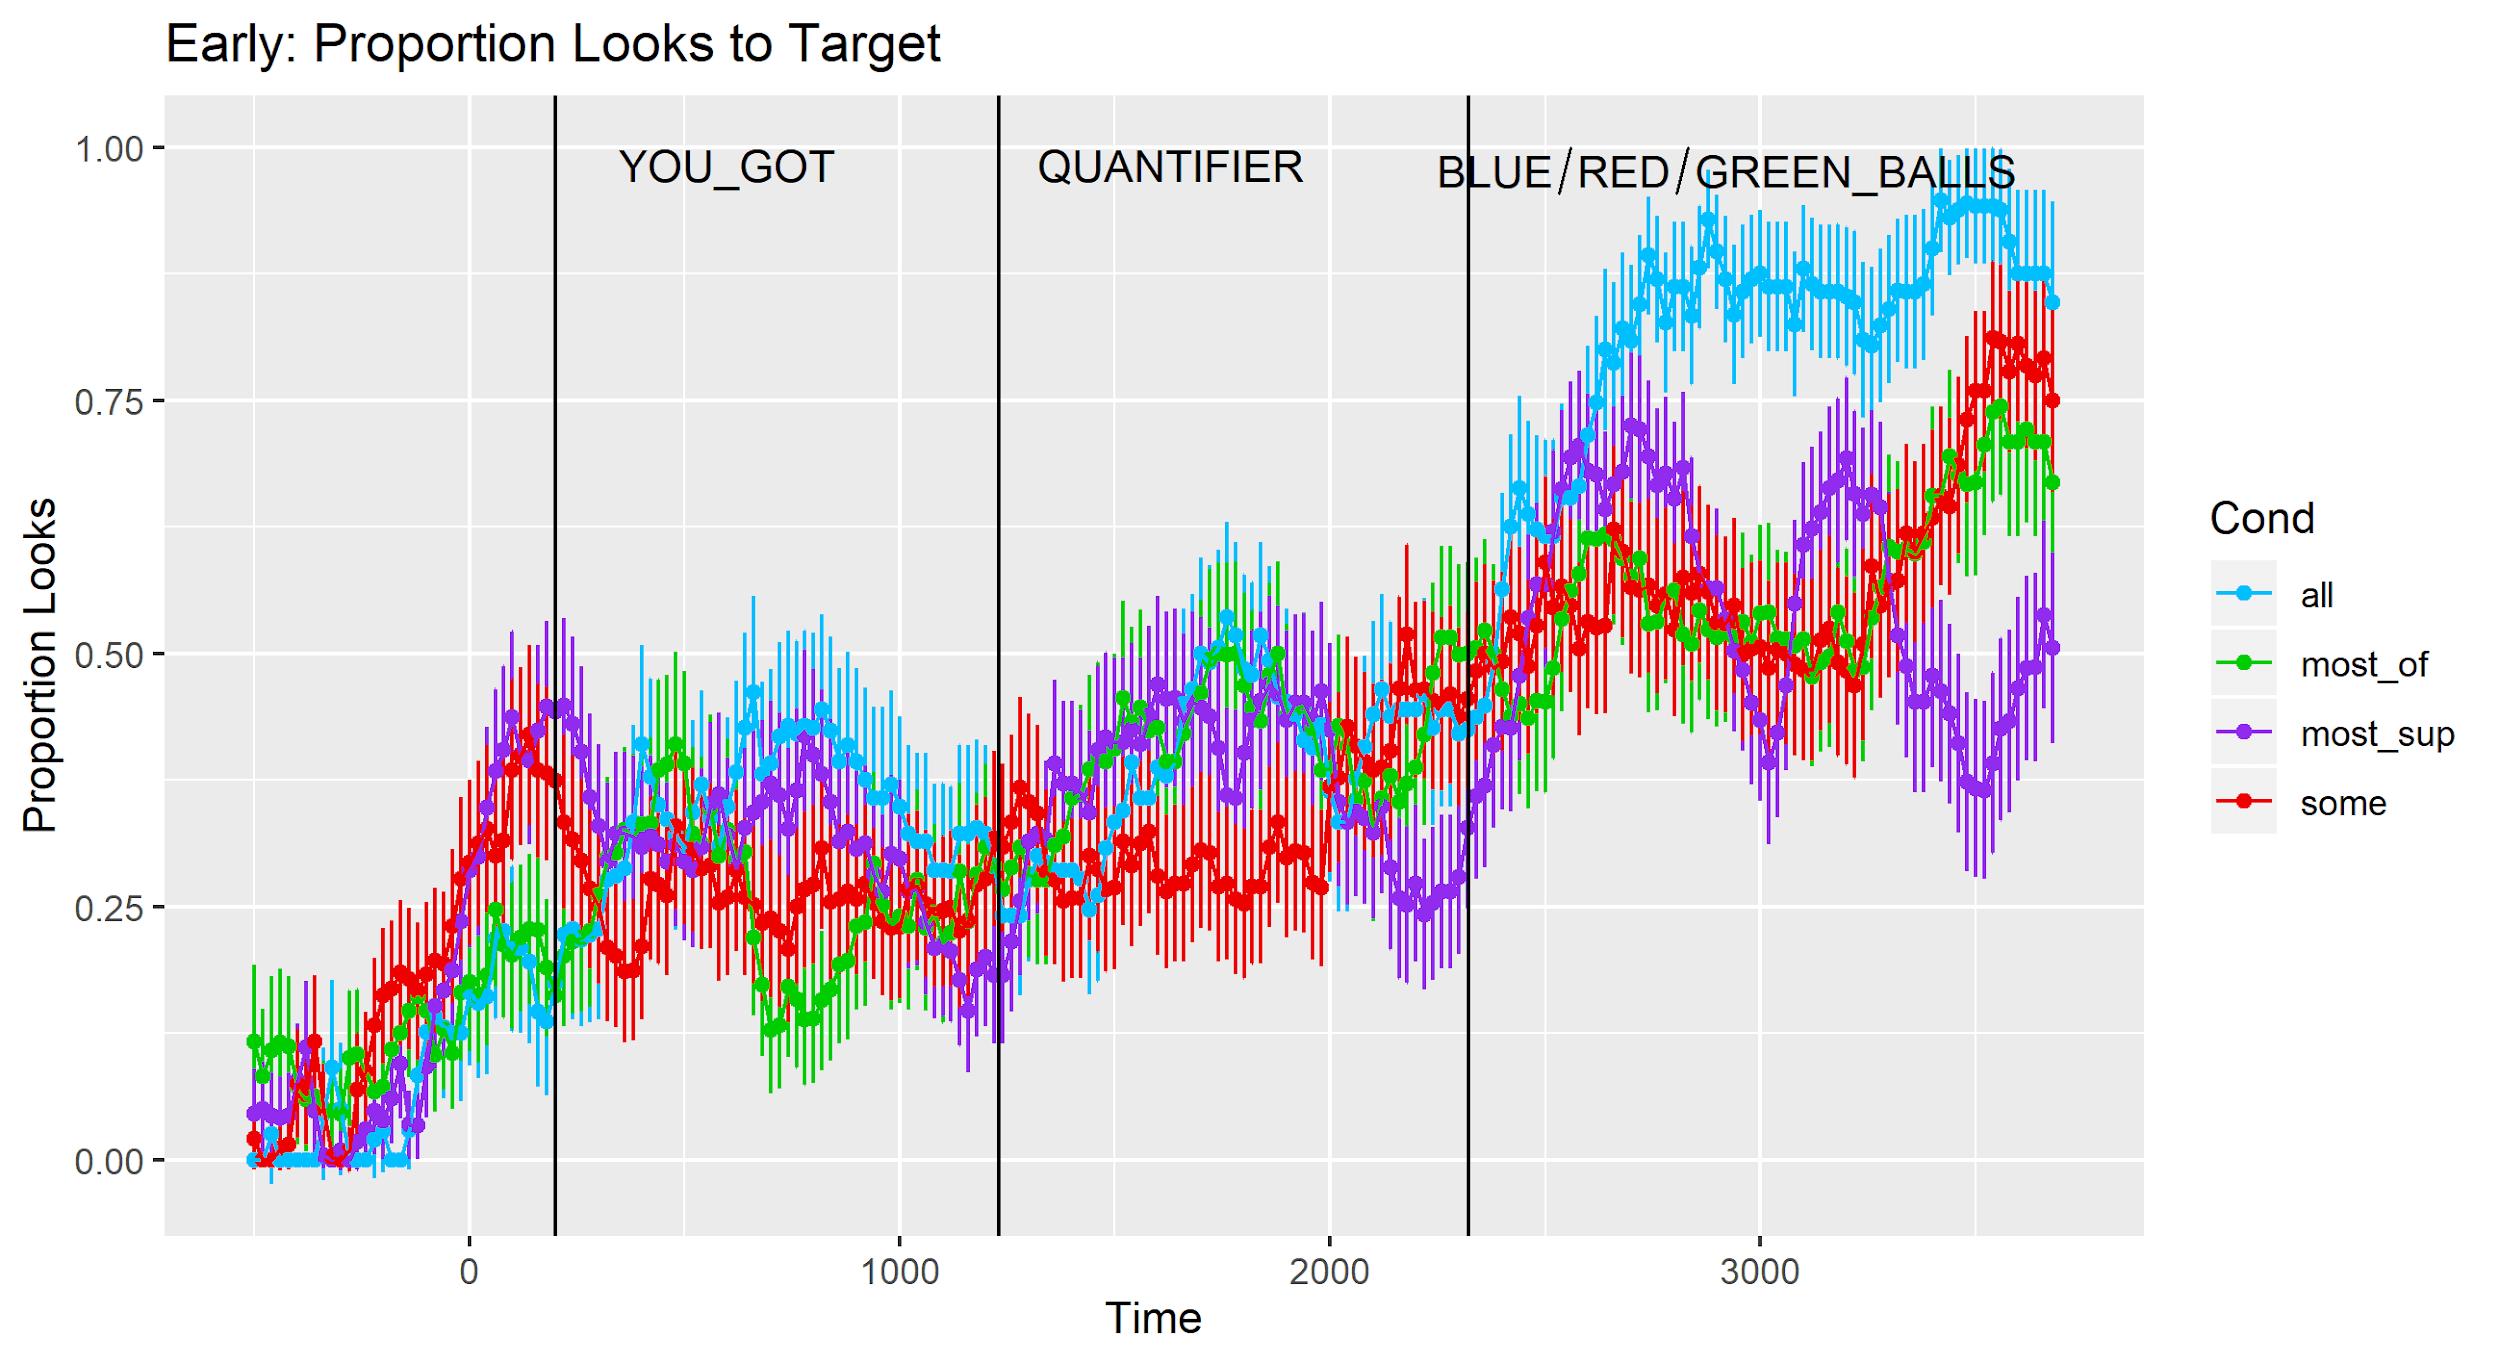
\includegraphics[width=\textwidth]{draftsinfonijarevisedfinal1-img017.png}
 \begin{tabularx}{\textwidth}{C@{}C@{}C@{}C}
%  \lsptoprule
%   \midrule
  %\multicolumn{4}{l}{\textbf{EARLY}}\\
%   \multicolumn{4}{l}{}\\
%   \midrule
\multicolumn{4}{c}{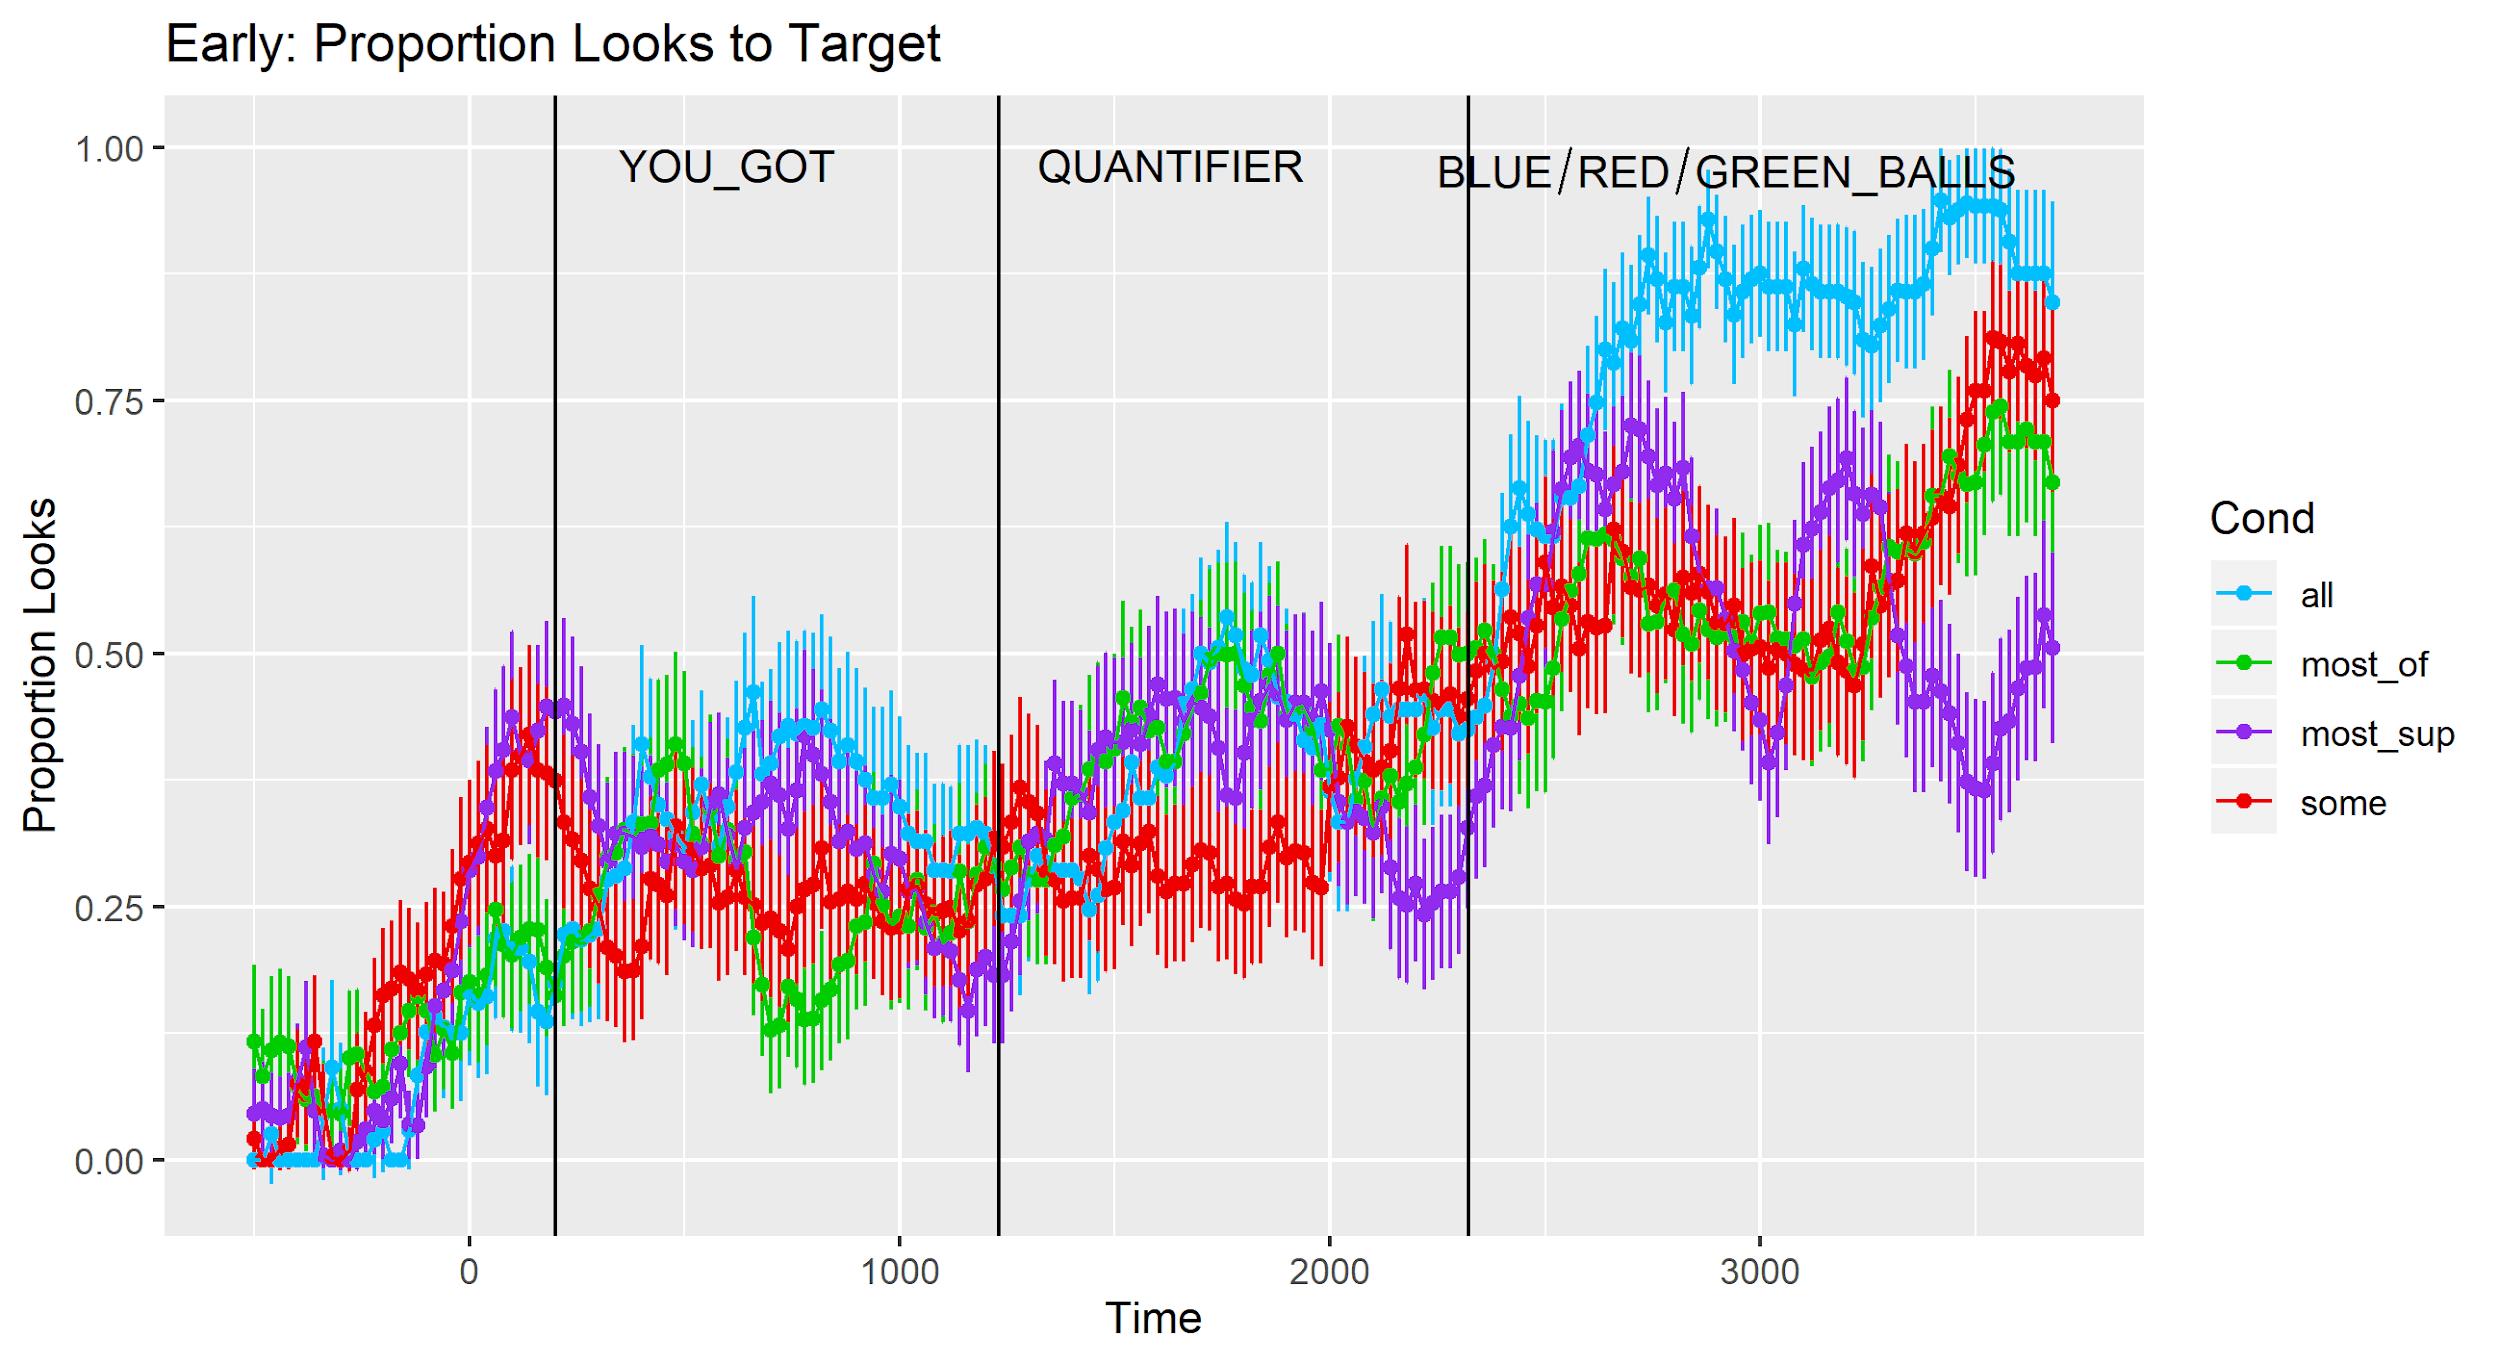
\includegraphics[width=\textwidth]{draftsinfonijarevisedfinal1-img017.png}}\\
        Preview & `You got' & Quantifier (†)& Color\,+\,`balls'\\
  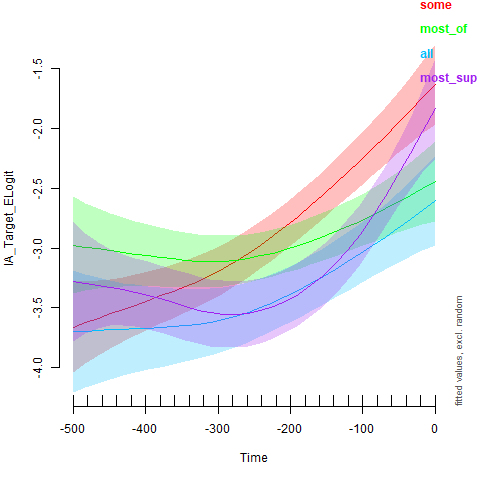
\includegraphics[width=0.2\textwidth]{draftsinfonijarevisedfinal1-img018.png}  &
 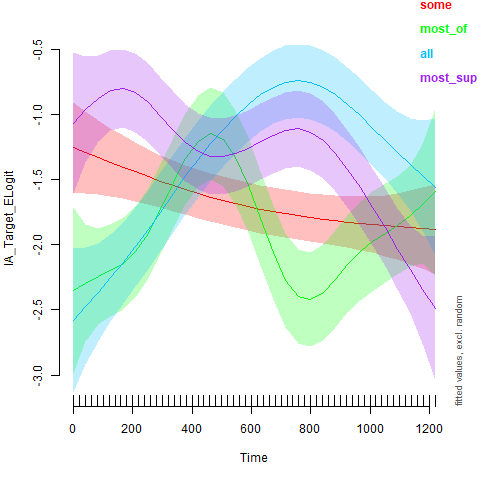
\includegraphics[width=0.2\textwidth]{draftsinfonijarevisedfinal1-img019.png}  &
 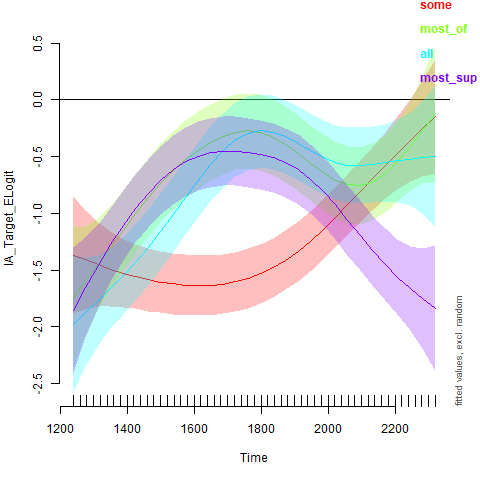
\includegraphics[width=0.2\textwidth]{draftsinfonijarevisedfinal1-img020.png}  &
 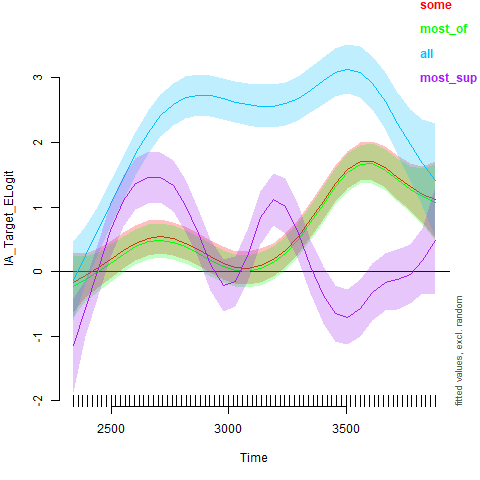
\includegraphics[width=0.2\textwidth]{draftsinfonijarevisedfinal1-img021.png}\\
 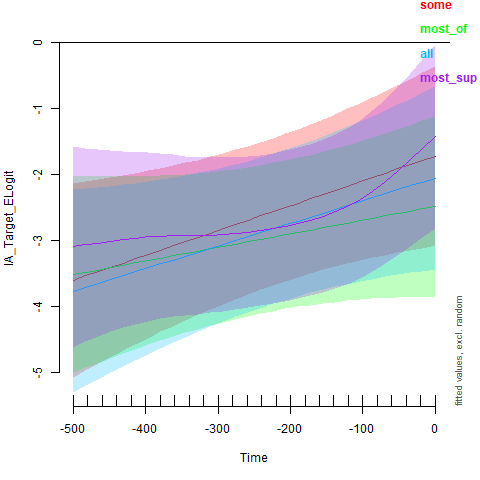
\includegraphics[width=0.2\textwidth]{draftsinfonijarevisedfinal1-img022.png}  &
 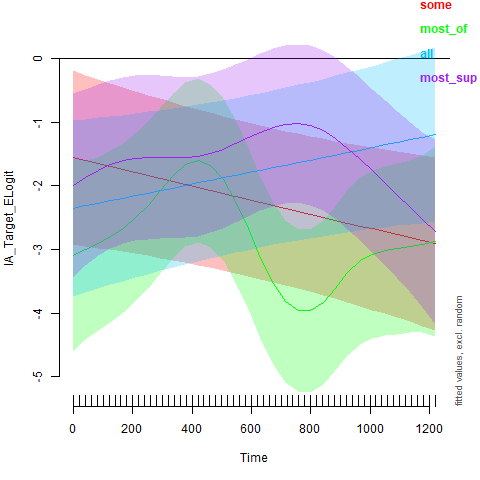
\includegraphics[width=0.2\textwidth]{draftsinfonijarevisedfinal1-img023.png}  &
 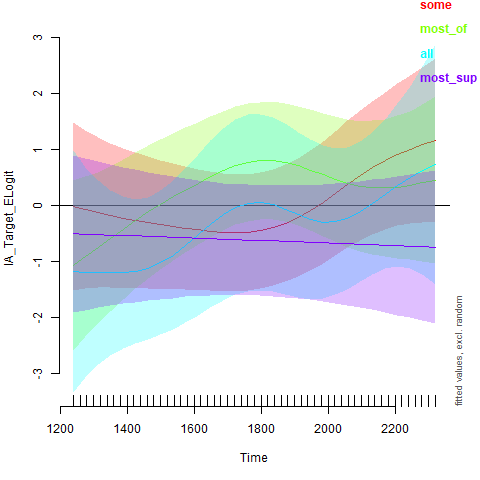
\includegraphics[width=0.2\textwidth]{draftsinfonijarevisedfinal1-img024.png}  &
 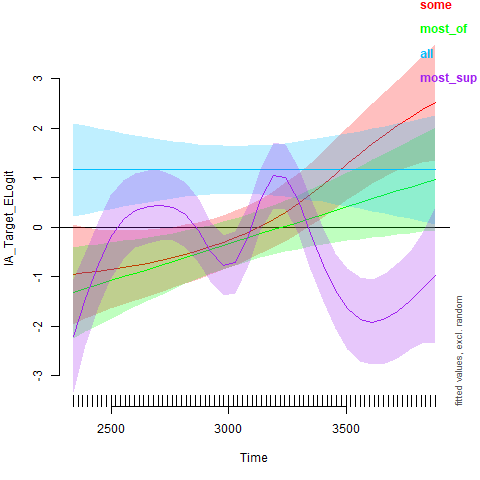
\includegraphics[width=0.2\textwidth]{draftsinfonijarevisedfinal1-img025.png} \\
 
 {\footnotesize{\mygraybox{\textsc{\textcolor[rgb]{0.6,0.0,1.0}{most\textsubscript{sup}}}\textcolor[rgb]{0.6,0.0,1.0}{} {\textgreater} \textsc{\textcolor[rgb]{0.41568628,0.65882355,0.30980393}{most-of}}}}}&
 {\footnotesize\textsc{\textcolor[rgb]{0.6,0.0,1.0}{most\textsubscript{sup}}}\textcolor[rgb]{0.6,0.0,1.0}{} = \textsc{\textcolor[rgb]{0.2901961,0.5254902,0.9098039}{all}}}&
 {\footnotesize\mygraybox{\textsc{\textcolor[rgb]{0.6,0.0,1.0}{most\textsubscript{sup}}}\textcolor[rgb]{0.6,0.0,1.0}{} = \textsc{\textcolor[rgb]{0.2901961,0.5254902,0.9098039}{all}}}}&
 {\footnotesize\textsc{\textcolor[rgb]{0.6,0.0,1.0}{most\textsubscript{sup}}}\textcolor[rgb]{0.6,0.0,1.0}{} {\textless} \textsc{\textcolor[rgb]{0.2901961,0.5254902,0.9098039}{all}}}\\
 
 {\footnotesize\mygraybox{\textsc{\textcolor{red}{Some}}\textcolor{red}{} {\textgreater} \textsc{\textcolor[rgb]{0.41568628,0.65882355,0.30980393}{most-of}}}}&
 {\footnotesize\mygraybox{\textsc{\textcolor[rgb]{0.6,0.0,1.0}{most\textsubscript{sup}}}\textcolor[rgb]{0.6,0.0,1.0}{} {\textgreater} \textsc{\textcolor[rgb]{0.41568628,0.65882355,0.30980393}{most-of}}}}&
 {\footnotesize\textsc{\textcolor[rgb]{0.6,0.0,1.0}{most\textsubscript{sup}}}\textcolor[rgb]{0.6,0.0,1.0}{} {\textless}  \textsc{\textcolor[rgb]{0.41568628,0.65882355,0.30980393}{most-of}}}&
 {\footnotesize\textsc{\textcolor[rgb]{0.6,0.0,1.0}{most\textsubscript{sup}}}\textcolor[rgb]{0.6,0.0,1.0}{} = \textsc{\textcolor[rgb]{0.41568628,0.65882355,0.30980393}{most-of}}}\\
 
 {\footnotesize{\textsc{\textcolor[rgb]{0.6,0.0,1.0}{most\textsubscript{sup}}}\textcolor[rgb]{0.6,0.0,1.0}{} = \textsc{\textcolor[rgb]{0.2901961,0.5254902,0.9098039}{all}}\textcolor[rgb]{0.2901961,0.5254902,0.9098039}{} = \textsc{\textcolor{red}{Some}}}}&
 {\footnotesize\mygraybox{\textsc{\textcolor[rgb]{0.6,0.0,1.0}{most\textsubscript{sup}}}\textcolor[rgb]{0.6,0.0,1.0}{} {\textgreater} \textsc{\textcolor{red}{Some}}}}&
 {\footnotesize\textsc{\textcolor[rgb]{0.6,0.0,1.0}{most\textsubscript{sup}}}\textcolor[rgb]{0.6,0.0,1.0}{} {\textless} \textsc{\textcolor{red}{Some}}}&
 {\footnotesize\textsc{\textcolor[rgb]{0.6,0.0,1.0}{most\textsubscript{sup}}}\textcolor[rgb]{0.6,0.0,1.0}{} {\textless} \textsc{\textcolor{red}{Some}}}\\
 
 &
 {\footnotesize\mygraybox{\textsc{\textcolor{red}{Some}}\textcolor{red}{} {\textgreater} \textsc{\textcolor[rgb]{0.41568628,0.65882355,0.30980393}{most-of}}}}&
 {\footnotesize{\textsc{\textcolor{red}{Some}}\textcolor{red}{ }=}\textsc{\textcolor[rgb]{0.2901961,0.5254902,0.9098039}{all}}\mygraybox{\textcolor[rgb]{0.2901961,0.5254902,0.9098039}{}=\textsc{\textcolor[rgb]{0.41568628,0.65882355,0.30980393}{most-of}}}}&
 {\footnotesize\textsc{\textcolor{red}{Some}}\textcolor{red}{ } {\textless} \textsc{\textcolor[rgb]{0.2901961,0.5254902,0.9098039}{all}}}\\
 
 &
 {\footnotesize\textsc{\textcolor{red}{Some}}\textcolor{red}{} = \textsc{\textcolor[rgb]{0.2901961,0.5254902,0.9098039}{all}}}&&
 {\footnotesize\textsc{\textcolor{red}{Some}}\textcolor{red}{ } {\textgreater} \textsc{\textcolor[rgb]{0.41568628,0.65882355,0.30980393}{most-of}}}\\
%  \thead{\colorbox{black!10}{\textsc{\textcolor[rgb]{0.6,0.0,1.0}{most\textsubscript{sup}}}\textcolor[rgb]{0.6,0.0,1.0}{}{\textgreater} \textsc{\textcolor[rgb]{0.41568628,0.65882355,0.30980393}{most-of}}}\\
%  \colorbox{black!10}{\textsc{\textcolor{red}{Some}}\textcolor{red}{}{\textgreater}\textsc{\textcolor[rgb]{0.41568628,0.65882355,0.30980393}{most-of}}}\\
%  \textsc{\textcolor[rgb]{0.6,0.0,1.0}{most\textsubscript{sup}}}\textcolor[rgb]{0.6,0.0,1.0}{}= \textsc{\textcolor[rgb]{0.2901961,0.5254902,0.9098039}{all}}\textcolor[rgb]{0.2901961,0.5254902,0.9098039}{}=\textsc{\textcolor{red}{Some}}} &
%  \thead{\textsc{\textcolor[rgb]{0.6,0.0,1.0}{most\textsubscript{sup}}}\textcolor[rgb]{0.6,0.0,1.0}{}= \textsc{\textcolor[rgb]{0.2901961,0.5254902,0.9098039}{all}}\\
%  \colorbox{black!10}{\textsc{\textcolor[rgb]{0.6,0.0,1.0}{most\textsubscript{sup}}}\textcolor[rgb]{0.6,0.0,1.0}{}{\textgreater}\textsc{\textcolor[rgb]{0.41568628,0.65882355,0.30980393}{most-of}}}\\
%  \colorbox{black!10}{\textsc{\textcolor[rgb]{0.6,0.0,1.0}{most\textsubscript{sup}}}\textcolor[rgb]{0.6,0.0,1.0}{}{\textgreater}\textsc{\textcolor{red}{Some}}}\\
%  \colorbox{black!10}{\textsc{\textcolor{red}{Some}}\textcolor{red}{}{\textgreater} \textsc{\textcolor[rgb]{0.41568628,0.65882355,0.30980393}{most-of}}}\\
%  \textsc{\textcolor{red}{Some}}\textcolor{red}{}= \textsc{\textcolor[rgb]{0.2901961,0.5254902,0.9098039}{all}}} &
%  \thead{\colorbox{black!10}{\textsc{\textcolor[rgb]{0.6,0.0,1.0}{most\textsubscript{sup}}}\textcolor[rgb]{0.6,0.0,1.0}{}= \textsc{\textcolor[rgb]{0.2901961,0.5254902,0.9098039}{all}}}\\
% \textsc{\textcolor[rgb]{0.6,0.0,1.0}{most\textsubscript{sup}}}\textcolor[rgb]{0.6,0.0,1.0}{}{\textless} \textsc{\textcolor[rgb]{0.41568628,0.65882355,0.30980393}{most-of}}\\
% \textsc{\textcolor[rgb]{0.6,0.0,1.0}{most\textsubscript{sup}}}\textcolor[rgb]{0.6,0.0,1.0}{}{\textless} \textsc{\textcolor{red}{Some}}\\
% \textsc{\textcolor{red}{Some}}\textcolor{red}{ }=\textsc{\textcolor[rgb]{0.2901961,0.5254902,0.9098039}{all}}\colorbox{black!10}{\textcolor[rgb]{0.2901961,0.5254902,0.9098039}{}=\textsc{\textcolor[rgb]{0.41568628,0.65882355,0.30980393}{most-of}}}} & 
%  \thead{\textsc{\textcolor[rgb]{0.6,0.0,1.0}{most\textsubscript{sup}}}\textcolor[rgb]{0.6,0.0,1.0}{}{\textless} \textsc{\textcolor[rgb]{0.2901961,0.5254902,0.9098039}{all}}\\
% \textsc{\textcolor[rgb]{0.6,0.0,1.0}{most\textsubscript{sup}}}\textcolor[rgb]{0.6,0.0,1.0}{}= \textsc{\textcolor[rgb]{0.41568628,0.65882355,0.30980393}{most-of}}\\
% \textsc{\textcolor[rgb]{0.6,0.0,1.0}{most\textsubscript{sup}}}\textcolor[rgb]{0.6,0.0,1.0}{}{\textless} \textsc{\textcolor{red}{Some}}\\
% \textsc{\textcolor{red}{Some}}\textcolor{red}{ }{\textless} \textsc{\textcolor[rgb]{0.2901961,0.5254902,0.9098039}{all}}\\
% \textsc{\textcolor{red}{Some}}\textcolor{red}{ }{\textgreater}\textsc{\textcolor[rgb]{0.41568628,0.65882355,0.30980393}{most-of}}
% }\\
 \end{tabularx}
\end{figure}

Strikingly, there are differences between the quantifiers already during Preview and in the `You got' window. An
exploratory analysis is needed to find out what drove the differences. Perhaps it was some property of the previous
trial such as the quantifier, the location of the target (left, center, right) or the numerosities of the sets. Or perhaps
this reflects the anticipation of which sentence would best describe the display given that in the \textsc{late} condition,
there are no differences at Preview, but the differences start at `You got' such that \textsc{most-of} and
\textsc{some} get more looks than \textsc{most\textsubscript{sup}}.\footnote{ A reviewer
objects to this saying that it is unlikely that the participants would try to guess the upcoming quantifier or were
clairvoyant. But my suggestion is that the big-set bias has consequences for the mental representation of the
description of the visual scene. See \citet{huettig2011looking} for the explanation of the interaction between the visual
stimuli and higher order cognitive biases as induced by task goals and language. In the \textsc{late} condition, a salient
visual cue is absent and the looks do not diverge during Preview. In the \textsc{early} condition, the target set pops out and
may bias some mental description of the scene, which is additionally affected by the memory of any salient features of
the previous trial.}

Crucially for the goals of the experiment, in the quantifier window the unexpected trends from the previous windows do
not persist. Instead, I find that the predictions have been met: with \textsc{most\textsubscript{sup}} there were
fewer looks to the target than with \textsc{some} and \textsc{most-of}. This is the prediction
`\textsc{most\textsubscript{sup}} {\textless} \textsc{most-of}, \textsc{all}' in Table \ref{tom:tab:1:predictions}. (There is no significant
difference between \textsc{most\textsubscript{sup}} and \textsc{all}, which was unpredicted, however, \textsc{some} is
also not significantly different from \textsc{all} and it can be seen in the plot with random effects that there is a
lot of variation with \textsc{all}). 

I predicted that the lower proportion of looks to the target with \textsc{most\textsubscript{sup}} than with
\textsc{most-of} should be due the fact that its semantics requires two comparisons (between the target and the two
color sets in the lower chamber) while with \textsc{most-of} one comparison is required (between the lower and upper
subsets of the partitioned set). The question was whether with \textsc{some} the looks to the target would be the same
as with \textsc{most\textsubscript{sup}} suggesting that the processing of the scalar implicature does not happen in
the quantifier window. I find that this is not the case: there are more looks to the target with \textsc{some} than
with \textsc{most\textsubscript{sup}} and \textsc{some} is no different from \textsc{most-of} (and \textsc{all}). This
result is compatible with the prediction `\textsc{some-not-all} {\textgreater} \textsc{most\textsubscript{sup}}' in
Table \ref{tom:tab:1:predictions}, meaning that the scalar implicature, `some-but-not-all', has already been processed in the quantifier
window. I find no support for the alternative, that first the literal meaning of \textit{some}, `some-and-possibly-all', is processed, `\textsc{some-possibly-all} = \textsc{most\textsubscript{sup}}' in Table \ref{tom:tab:1:predictions}.

It was also predicted that in the \textsc{early} condition in the quantifier window \textsc{some-not-all} would get more looks to
the target than \textsc{most-of} (`\textsc{some-not-all} {\textgreater} \textsc{most-of}' in Table \ref{tom:tab:1:predictions}), but instead we
find that \textsc{some} is no different from \textsc{most-of} (`\textsc{some} = \textsc{most-of}' in Figure \ref{tom:tab:2:early}) – we do
find evidence for this effect but in the next region.

The prediction for the color adjective window was `\textsc{some-not-all} {\textgreater} \textsc{most-of}' if \textsc{most-of} requires more looks between the two partitioned sets than \textsc{some} in order to establish the total set of the balls in the target color for the Subtraction procedure, (\ref{tom:ex:subtraction}). I hypothesized that the proportion of looks to the target with
\textsc{most-of} could be as low as with \textsc{most\textsubscript{sup}}, which is what we find
(`\textsc{most\textsubscript{sup}} = \textsc{most-of}' in Figure \ref{tom:tab:2:early}). However, looking at the plots we see that the
difference between \textsc{most-of} and \textsc{some} is rather small; there are more looks to the target with \textsc{some} 
at the very beginning and mostly at the end of the region. The trajectory for \textsc{most-of} is quite different
than for \textsc{most\textsubscript{sup}}, where the looks diverge between the target and the distractors.
Still, the proportion of looks to the target within the whole region is as low with \textsc{most-of} as with
\textsc{most\textsubscript{sup}}, which is consistent with a higher number of processing steps involved in the
Subtraction procedure in contrast with the direct Selection procedure.

The results for the \textsc{late} condition are presented in Figure \ref{tom:tab:3:late}. In the \textsc{late} condition, there are also effects of Quantifier in each time window (Preview: $\chi^2=18.4, \text{df}=9, p=0.009$; `You got': $\chi^2=113.12, \text{df}=9,
p<0.0001$; the quantifier: $\chi^2=112.61, \text{df}=9, p<0.0001$; the color window:
$\chi^2=163.25, \text{df}=9, p<0.0001$). In contrast to the \textsc{early} condition, in the Preview window multiple
comparisons show no significant differences. In other windows pairwise comparisons reveal the following differences
(\textit{p}{}-values include the Bonferroni correction for multiple comparisons):

In the `You got' window, in the \textsc{late} condition, \textsc{most\textsubscript{sup}} got fewer looks to the target than all
the other conditions (\textsc{some}, $\beta =0.847, \text{SE}=0.102, t=8.321, p<0.001$,
\textsc{all}, $\beta =2.754, \text{SE}=0.855, t=3.223, p=0.005$, \textsc{most-of}, $\beta =1.274, \text{SE}=0.108,
t=11.749, p<0.0001$). \textsc{some} received fewer looks to the target than \textsc{most-of} ($\beta
=0.434, \text{SE}=0.102, t=4.258, p<0.0001$). As in the \textsc{early} condition, this result is unexpected
and requires an exploratory analysis. 

% \begin{figure}[h]
%     \centering
%     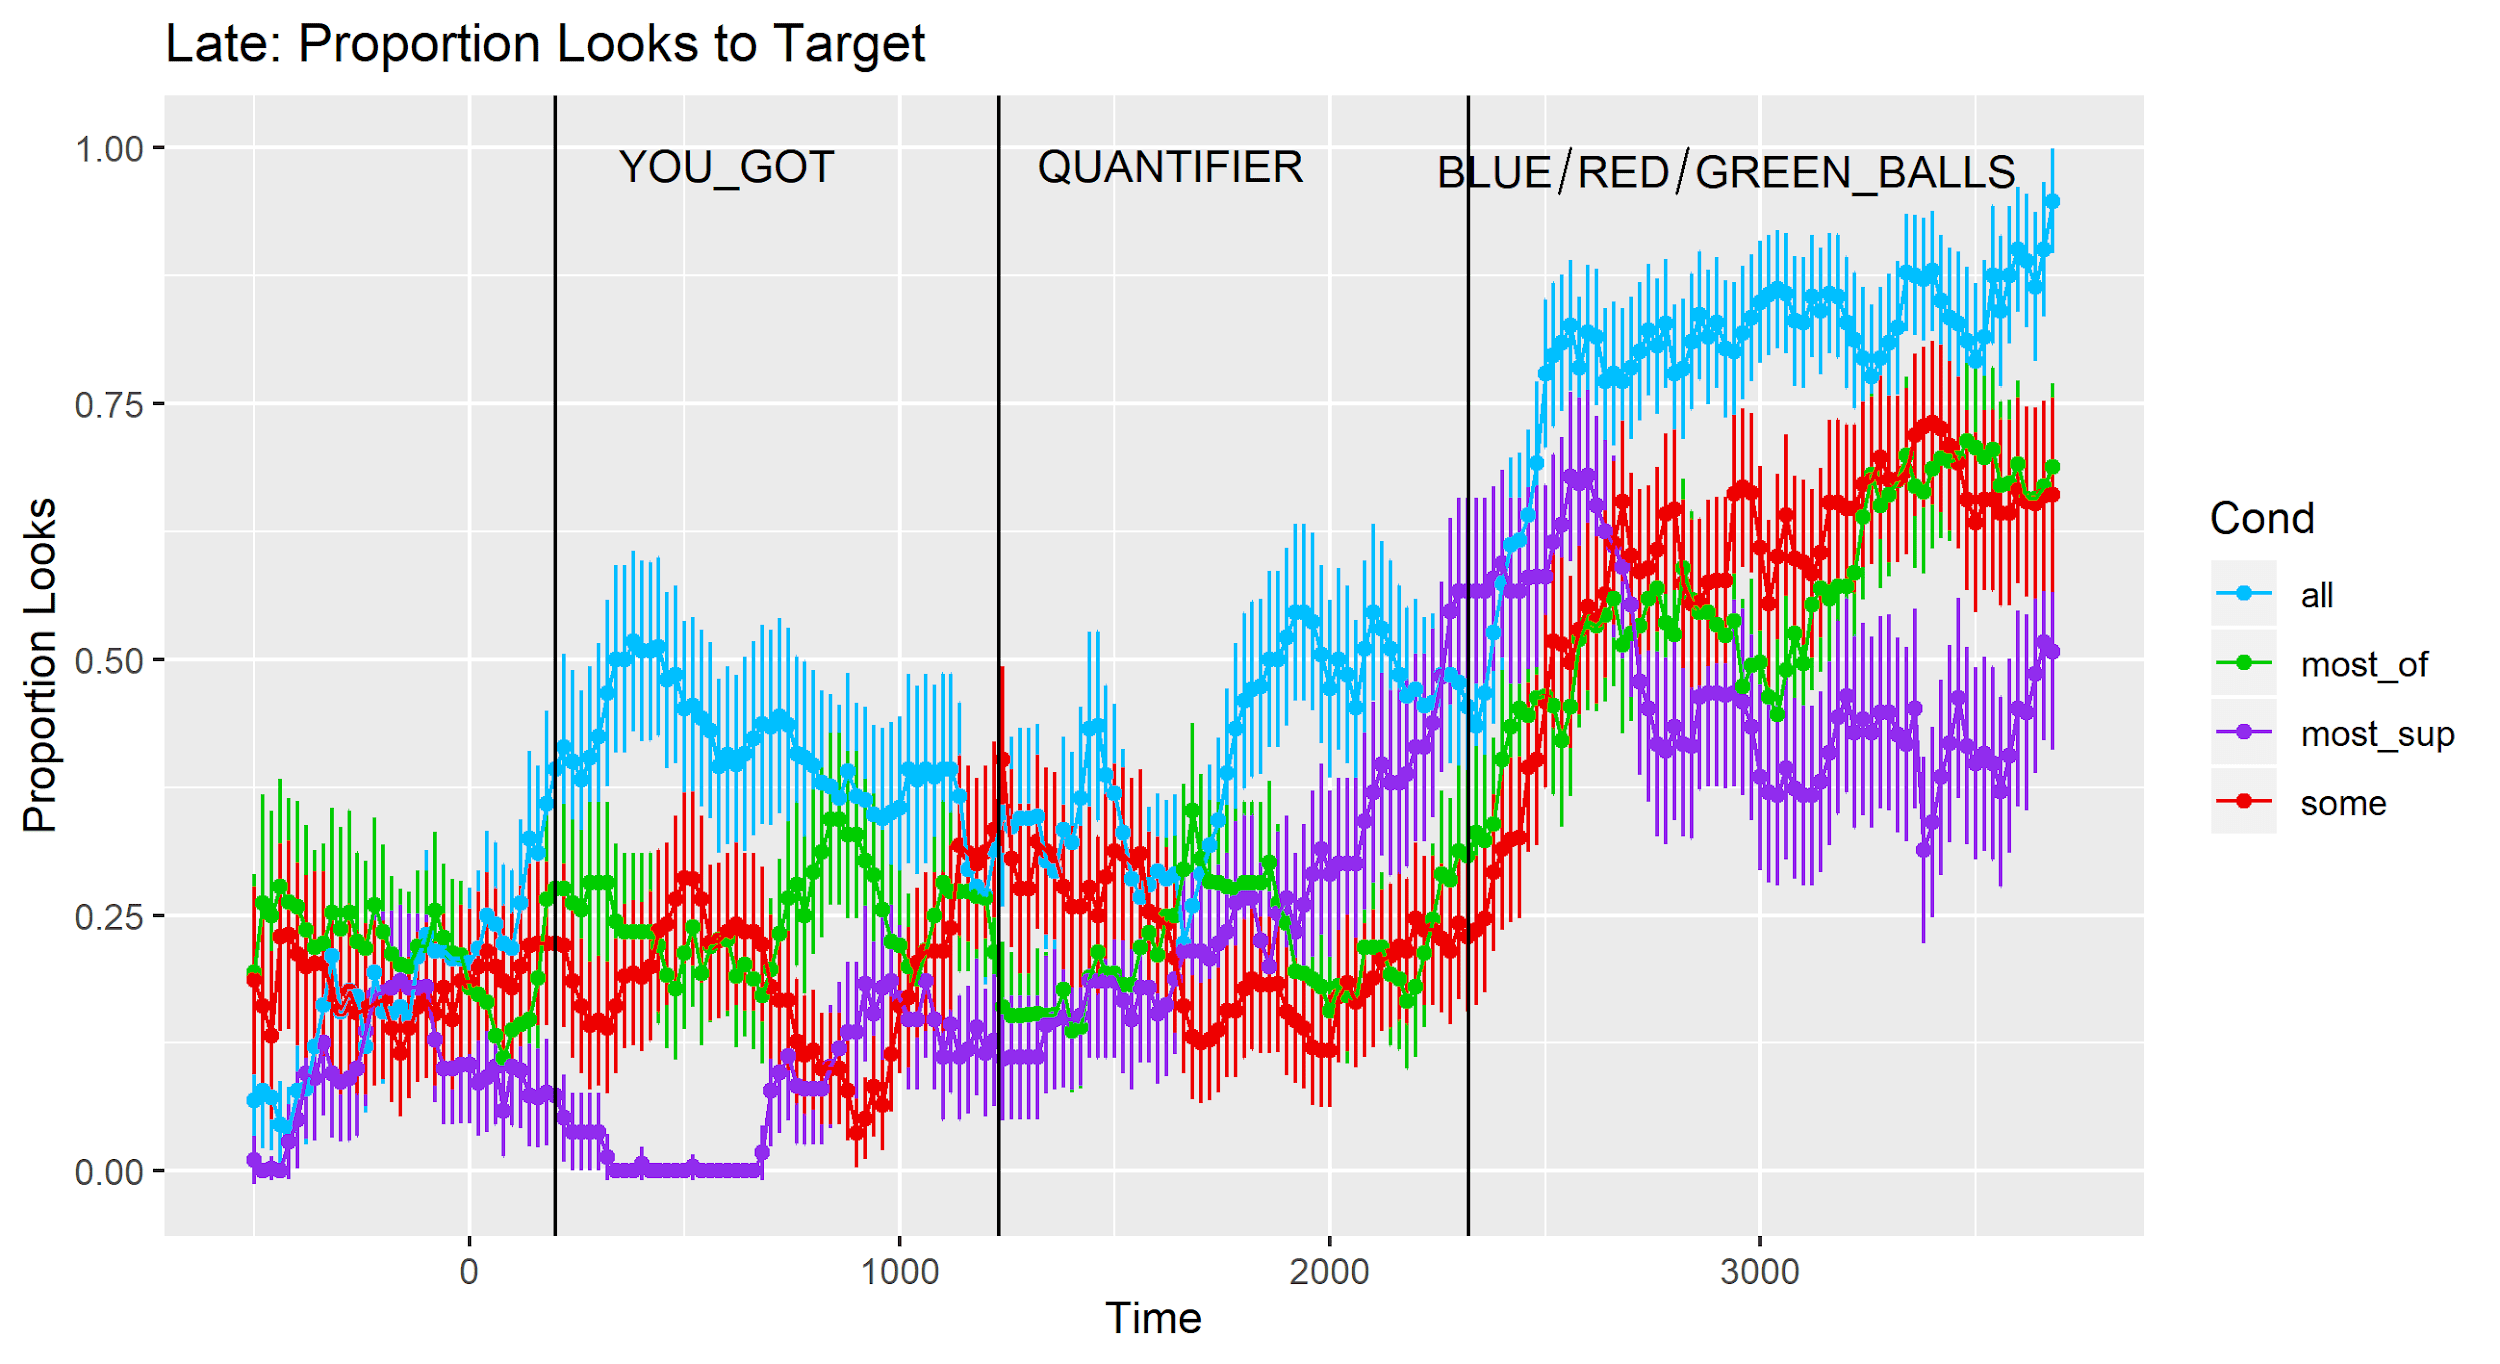
\includegraphics[width=0.95\textwidth]{draftsinfonijarevisedfinal1-img026.png}
%     \caption{ADD CAPTION}
%     \label{tom:fig:result-late}
% \end{figure}

\begin{figure}[p]\small
\centering
\caption{Results: \textsc{late} condition. (†) marks \textit{disambiguation}.}
\label{tom:tab:3:late}
 \begin{tabularx}{\textwidth}{C@{}C@{}C@{}C}
%  \lsptoprule
    % \midrule
  %\multicolumn{4}{l}{\textbf{LATE}}\\
%   \multicolumn{4}{l}{}\\
%   \midrule
\multicolumn{4}{c}{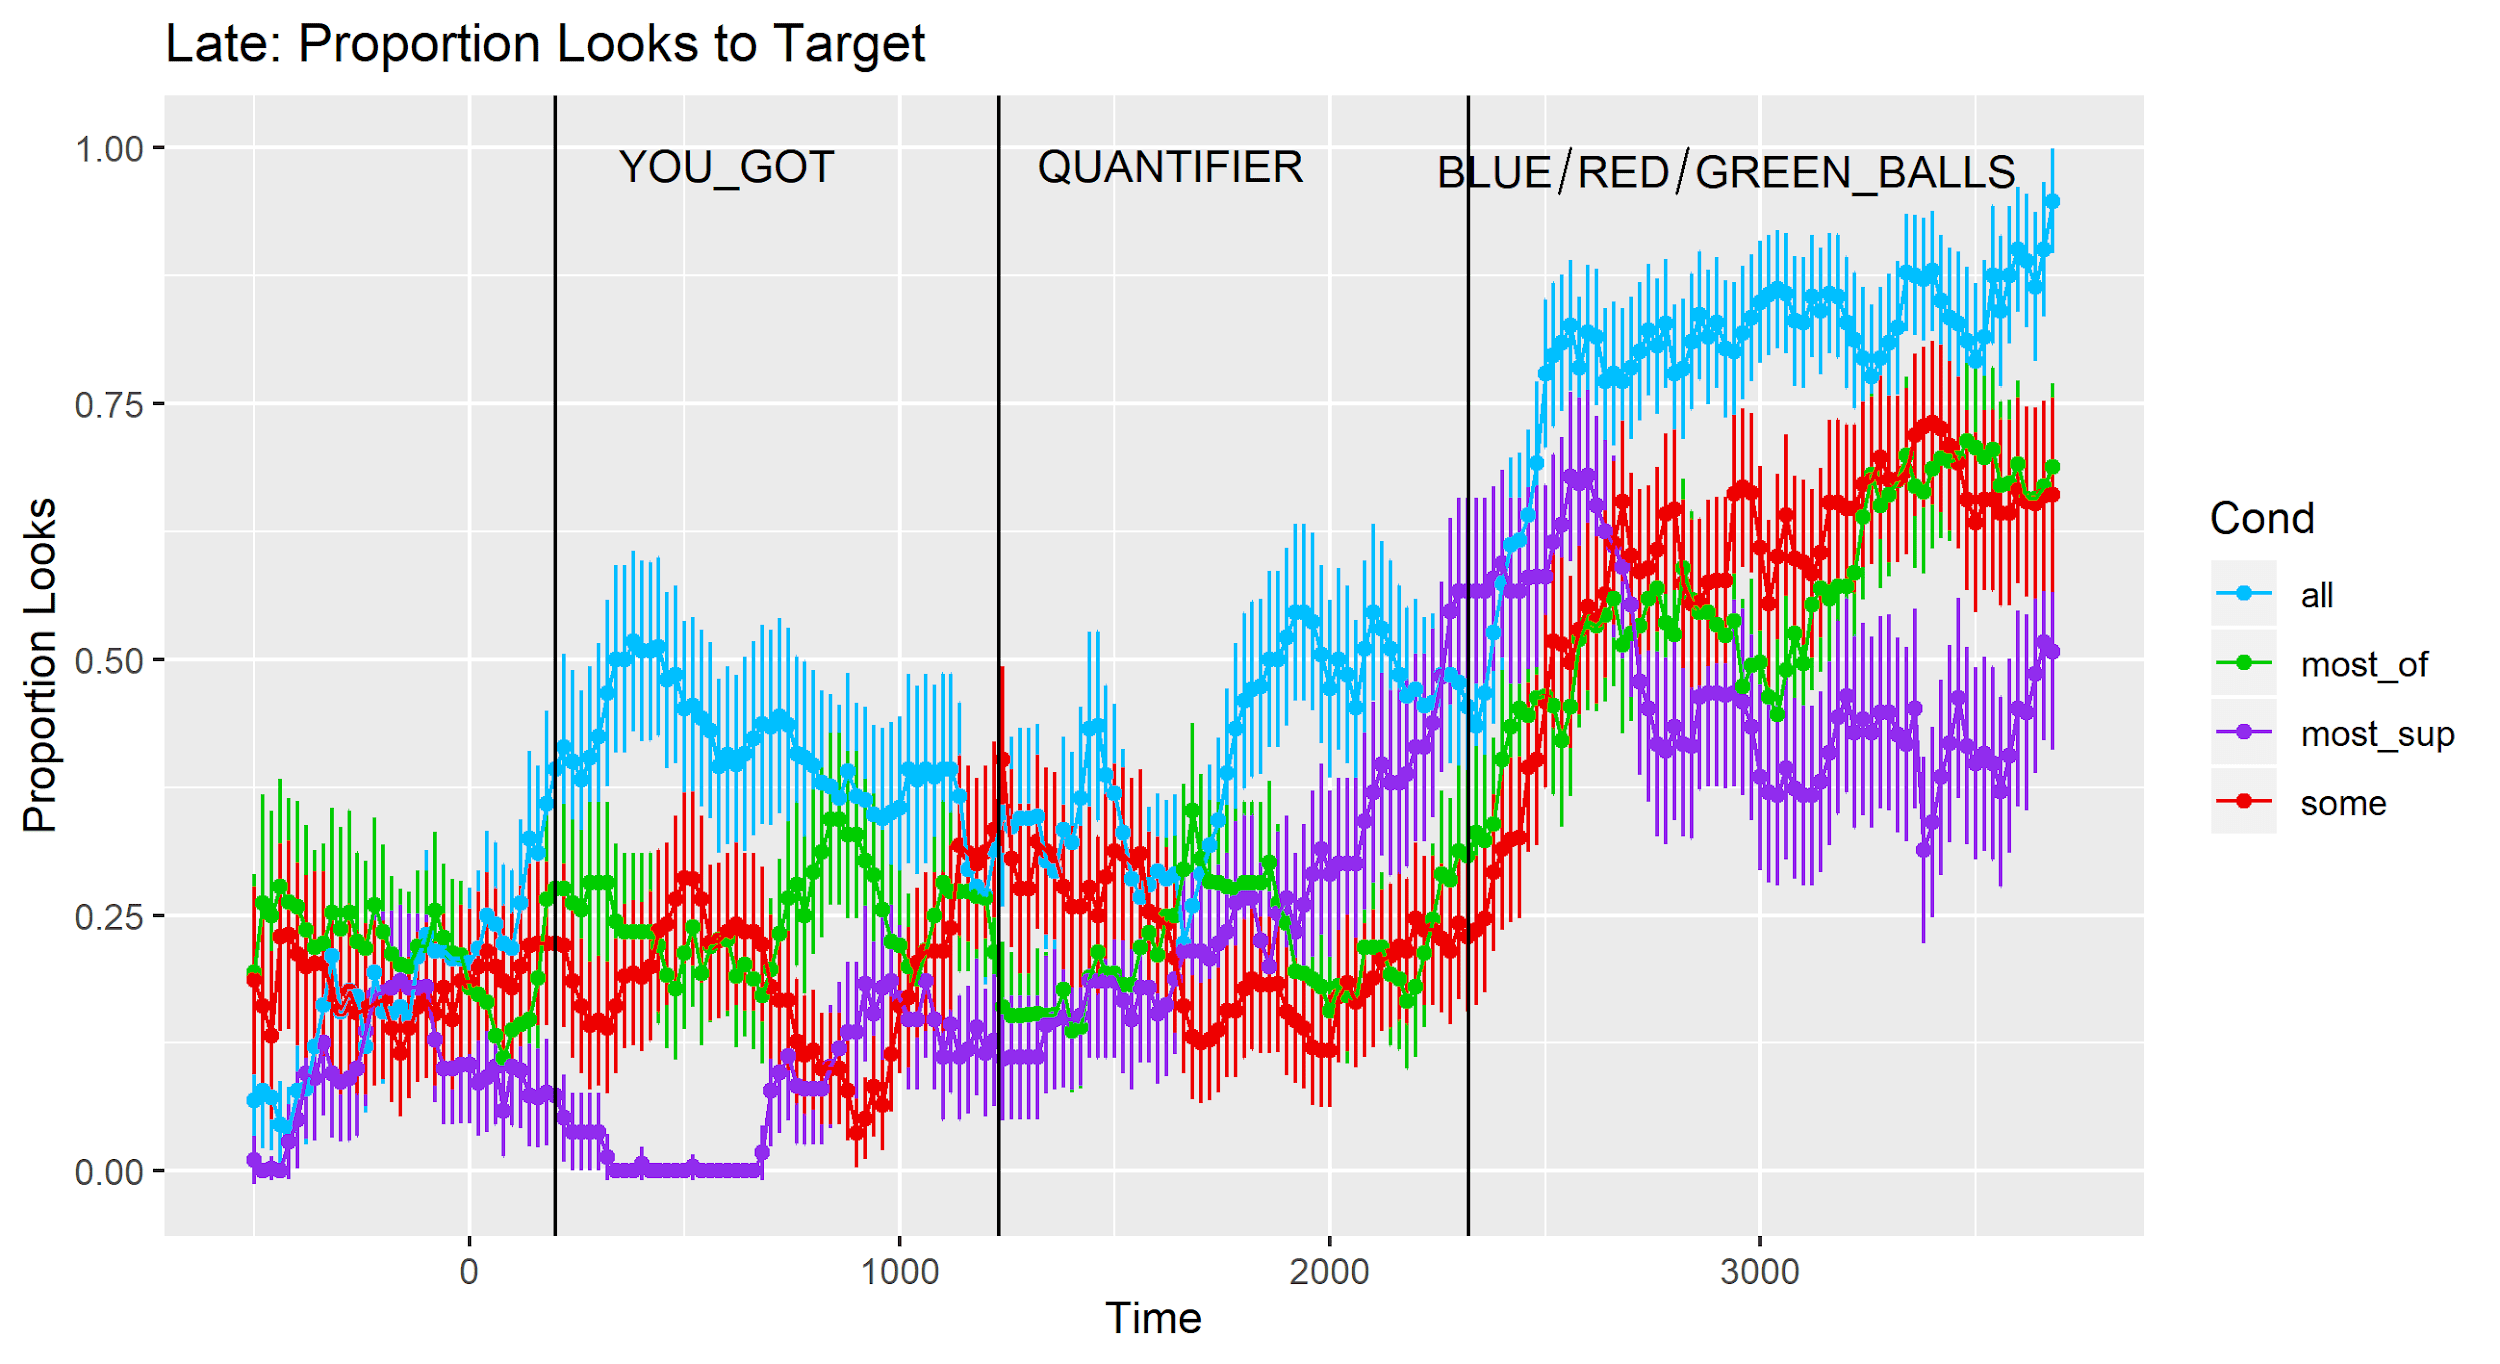
\includegraphics[width=0.95\textwidth]{draftsinfonijarevisedfinal1-img026.png}}\\
        Preview & `You got' & Quantifier& Color\,+\,`balls' (†)\\
  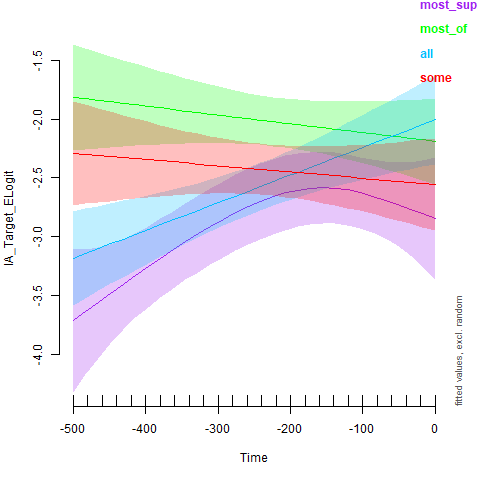
\includegraphics[width=0.2\textwidth]{draftsinfonijarevisedfinal1-img027.png}  &
 \includegraphics[width=0.2\textwidth]{draftsinfonijarevisedfinal1-img028.png}  &
 \includegraphics[width=0.2\textwidth]{draftsinfonijarevisedfinal1-img029.png}  &
 \includegraphics[width=0.2\textwidth]{draftsinfonijarevisedfinal1-img030.png}\\
 \includegraphics[width=0.2\textwidth]{draftsinfonijarevisedfinal1-img031.png}  &
 \includegraphics[width=0.2\textwidth]{draftsinfonijarevisedfinal1-img032.png}  &
 \includegraphics[width=0.2\textwidth]{draftsinfonijarevisedfinal1-img033.png}  &
 \includegraphics[width=0.2\textwidth]{draftsinfonijarevisedfinal1-img034.png} \\
 no differences&
 
 {\footnotesize\mygraybox{\textsc{\textcolor[rgb]{0.6,0.0,1.0}{most\textsubscript{sup}}}\textcolor[rgb]{0.6,0.0,1.0}{} {\textless} \textsc{\textcolor[rgb]{0.2901961,0.5254902,0.9098039}{all}}}}&
 {\footnotesize\mygraybox{\textsc{\textcolor[rgb]{0.6,0.0,1.0}{most\textsubscript{sup}}}\textcolor[rgb]{0.6,0.0,1.0}{} = \textsc{\textcolor[rgb]{0.2901961,0.5254902,0.9098039}{all}}}}&
 {\footnotesize\textsc{\textcolor[rgb]{0.6,0.0,1.0}{most\textsubscript{sup}}}\textcolor[rgb]{0.6,0.0,1.0}{} {\textless} \textsc{\textcolor[rgb]{0.2901961,0.5254902,0.9098039}{all}}}\\
 
&{\footnotesize\mygraybox{\textsc{\textcolor[rgb]{0.6,0.0,1.0}{most\textsubscript{sup}}}\textcolor[rgb]{0.6,0.0,1.0}{} {\textless} \textsc{\textcolor[rgb]{0.41568628,0.65882355,0.30980393}{most-of}}}}&
{\footnotesize\textsc{\textcolor[rgb]{0.6,0.0,1.0}{most\textsubscript{sup}}}\textcolor[rgb]{0.6,0.0,1.0}{} {\textgreater} \textsc{\textcolor[rgb]{0.41568628,0.65882355,0.30980393}{most-of}}}&
{\footnotesize\textsc{\textcolor[rgb]{0.6,0.0,1.0}{most\textsubscript{sup}}}\textcolor[rgb]{0.6,0.0,1.0}{} {\textless} \textsc{\textcolor[rgb]{0.41568628,0.65882355,0.30980393}{most-of}}}\\

&{\footnotesize\mygraybox{\textsc{\textcolor[rgb]{0.6,0.0,1.0}{most\textsubscript{sup}}}\textcolor[rgb]{0.6,0.0,1.0}{} {\textless} \textsc{\textcolor{red}{Some}}}}&
{\footnotesize\textsc{\textcolor[rgb]{0.6,0.0,1.0}{most\textsubscript{sup}}}\textcolor[rgb]{0.6,0.0,1.0}{} {\textgreater} \textsc{\textcolor{red}{Some}}}&
{\footnotesize\textsc{\textcolor[rgb]{0.6,0.0,1.0}{most\textsubscript{sup}}}\textcolor[rgb]{0.6,0.0,1.0}{} {\textless} \textsc{\textcolor{red}{Some}}}\\

&{\footnotesize\mygraybox{\textsc{\textcolor{red}{Some}}\textcolor{red}{ } = \textsc{\textcolor[rgb]{0.2901961,0.5254902,0.9098039}{all}}}}&
{\footnotesize\mygraybox{\textsc{\textcolor{red}{Some}}\textcolor{red}{ } = \textsc{\textcolor[rgb]{0.2901961,0.5254902,0.9098039}{all}}}}&
{\footnotesize\textsc{\textcolor{red}{Some}}\textcolor{red}{ } {\textless} \textsc{\textcolor[rgb]{0.2901961,0.5254902,0.9098039}{all}}}\\

&{\footnotesize\mygraybox{\textsc{\textcolor{red}{Some}}\textcolor{red}{ } {\textless} \textsc{\textcolor[rgb]{0.41568628,0.65882355,0.30980393}{most-of}}}}&
{\footnotesize\textsc{\textcolor{red}{Some}}\textcolor{red}{ } {\textgreater} 
\textsc{\textcolor[rgb]{0.41568628,0.65882355,0.30980393}{most-of}}}&
{\footnotesize\mygraybox{\textsc{\textcolor{red}{Some}}\textcolor{red}{ } = \textsc{\textcolor[rgb]{0.41568628,0.65882355,0.30980393}{most-of}}}}\\
 \end{tabularx}
\end{figure}


In the quantifier window, in the \textsc{late} condition, there were more looks to the target with
\textsc{most\textsubscript{sup}} than with \textsc{some} ($\beta =-0.562, \text{SE}=0.099, t=-5.688,
p<0.0001$) and than with \textsc{most-of} ($\beta =-0.838, \text{SE}=0.11, t=-7.606, p<0.0001$). This is in line with the prediction `\textsc{most\textsubscript{sup}} {\textgreater}
\textsc{all}, \textsc{most-of}, \textsc{some}' in Table \ref{tom:tab:1:predictions} (except that \textsc{most\textsubscript{sup}} is not
significantly different from \textsc{all}). We also find that there are more looks to the target with \textsc{some}
than with \textsc{most-of} ($\beta =-0.276, \text{SE}=0.103, t=-2.685, p=0.029$), which fits the prediction
`\textsc{some-not-all} {\textgreater} \textsc{most-of}' in Table \ref{tom:tab:1:predictions} and further indicates that with \textsc{some} there
is no delay in the processing of the scalar implicature.

I predicted that the latter effect would persist in the color window, but instead I find that \textsc{some} was no
different from \textsc{most-of}. This could be related to the low accuracy with \textit{some}, namely, participants who
accepted `some-not-all' as the description of the display (recall that I analyzed the looks with correct
responses only) nevertheless compared the numerosities of the different color sets. However, \textsc{some} had
significantly fewer looks to the target than \textsc{all} ($\beta =1.676, \text{SE}=0.276, t=6.071,
p<0.0001$). This effect, `\textsc{some-not-all} {\textless} \textsc{all}' was predicted to occur
already in the quantifier window, but we find it later.

In the color window, with \textsc{most\textsubscript{sup}} there were fewer looks to the target than with the other
quantifiers: \textsc{some} ($\beta =0.642, \text{SE}=0.097, t=6.641, p<0.0001$), \textsc{all}
($\beta =2.075, \text{SE}=0.277, t=7.505, p<0.0001$), and \textsc{most-of} ($\beta =0.46,
\text{SE}=0.101, t=4.536, p<0.0001$). This results is exactly as predicted: with
\textsc{most\textsubscript{sup}}, as the color adjective is heard the looks must be directed to the other two
color sets in order to make the comparisons to confirm that the target set is indeed the largest.


\section{Discussion and conclusions} 

The results of the current study contribute to the debate about the processing of the scalar implicature of the
quantifier \textit{some }during visual verification (\citealt{huang2009online,grodner2010some,degen2011making,huang2011logic,degen2016availability}) and provide novel predictions for experiments on the processing of \textit{some} in
comparison with other quantifiers in languages other than English. I find support for the claim in \citet{spychalska-msc}
that the Polish counterpart of \textit{some}, \textit{niektóre}, has a strong implicature – I find that the meaning
`some-not-all' is processed immediately as the disambiguating quantifier is heard. I compared \textit{niektóre} `some'
to \textit{większość} `most of' and \textit{najwięcej} (the superlative \textit{most}) and \textit{wszystkie
} `all'. In the prior visual world eye-tracking studies, \textit{some} and \textit{all} were compared on the
basis of the theory that these two quantifiers form a scale, so when \textit{some} is used instead of the stronger
\textit{all}, the inferred meaning is `some-not-all' (\citealt{horn1972,Levinson1983}, a.o.). However, the results of \citet{degen2011making,degen2016availability} showed that whether there is a delay in the processing of the `some-not-all'
meaning depends on whether the experiment contains alternative descriptions using number terms and not just
\textit{some} and \textit{all} (`You got some/all/two/three/four/five of the blue gumballs'). When those alternatives
are available the processing of the `some-not-all', implicature is delayed relative to the processing of the
meaning of \textit{all}. Without such alternatives, \textit{some} is not delayed relative to \textit{all}. 

In the current experiment, adopting the gumball paradigm of \citet{degen2011making,degen2016availability} alternative descriptions of
the visual scene contained the quantifiers \textit{most of} and the superlative \textit{most
}(\textit{most}\textsc{-sup}) because (i) they allowed for more specific predictions about the time course of the
looks to the target than just a comparison with \textit{all}, and (ii) two alternative strategies for \textit{most of}
could be tested. Specifically, the semantics of the superlative \textit{most} requires comparisons between the target
color set and the two other colors in the lower chambers of the ball machine, which I expected to elicit a
distinctive pattern of looks that would serve as the baseline for statistical comparisons (the displays were identical
for \textit{some}, \textit{most of} and \textit{most}\textsc{-sup}, but they had to be different for \textit{all}).
As in the study of \citet{degen2016availability} the quantifiers were compared with two types of displays, \textsc{early} and \textsc{late}
(Figures \ref{tom:fig:early}--\ref{tom:fig:late} in \sectref{tom:Predictions}). In the \textsc{early} condition, the quantifier in the stimulus sentence (`You got
some/all/most of/the most blue/red/green balls') disambiguated which set of the three sets of balls in
the bottom chambers was the target. In the \textsc{late} condition, the target was identifiable only when the color adjective was
heard. 

In the \textsc{early} condition, the results showed no delay for the Polish counterpart of \textit{some} as compared to
\textit{all} and \textit{most of}, as well as a higher proportion of looks to the target than with
\textit{most}\textsc{-sup}. I considered two alternatives in the predictions. On the one hand, if the
`some-not-all' meaning was processed early (at the point of hearing the quantifier), the identification of the
target set should be just as easy as with \textit{all}, given that the target set was partitioned and as such stood out
already during the preview. If, on the other hand, the `some-possibly-all' meaning was processed
first, the looks should be first directed to the unpartitioned sets as with \textit{most}\textsc{-sup}. The results
show support for the first option: the `some-not-all' meaning is processed early. In the \textsc{late} condition, I also
find evidence for the `some-not-all' interpretation in comparison with \textit{all} and \textit{most of}.

The second novel finding concerns the semantics of the majority quantifier \textit{most of}. \citet{pietroski2009meaning} and
\citet{lidz2011interface} propose that the verification of sentences like `You got most of the blue
balls' involves a procedure of subtraction (schematized in (\ref{tom:ex:subtraction}) vs. (\ref{tom:ex:selection}) in \sectref{tom:Predictions}). This procedure requires
multiple steps: estimate the superset (the blue balls remaining in the top chamber and the blue balls in the bottom
chamber), estimate the target set (the blue balls in the bottom chamber), subtract and compare the result with the
target. Subtraction involves more steps than direct comparison of two sets (\ref{tom:ex:selection} in \sectref{tom:Predictions}), so my hypothesis was
that I should find fewer looks to the target in the quantifier and color windows because of the continuing looks to
the top blue set in order to establish the total set. Indeed, in the color window there were significantly fewer looks
to the target than with both \textit{some} and \textit{all}; the proportion of looks was as low as in the
\textit{most}\textsc{-sup} condition. The low proportion of looks with \textit{most}\textsc{-sup} can be
directly linked to the superlative semantics requiring comparisons with the other color sets. \textit{most of} could be
verified by merely comparing the top and bottom numerosities of the partitioned set, but this simple comparison would
have elicited a similar proportion of looks to the target as with \textit{some}. The profiles of eye-movements with
\textit{some} and \textit{most of} looked similar but the proportion of looks to the target was lower with \textit{most
of} than with \textit{some}. In the \textsc{late} condition I also predicted fewer looks to the target with \textit{most of}
than with \textit{some} in both the quantifier and color windows, and this effect was observed in the quantifier
window.

The fact that the pattern of looks with \textit{most of} is compatible with the subtraction procedure and not with the
more efficient direct comparison procedure supports the hypothesis in \citet{pietroski2009meaning} and
\citet{lidz2011interface}
that the mind follows the “instructions” encoded in the lexical representation of quantifier meanings. They argue that
lexical semantics interfaces with the cognitive system, which means that lexical meanings require more fine grained
distinctions than just truth-conditions. The present experiment showing that with the same display there are
distinctive patterns of looks for the three Polish quantifiers \textit{some}, \textit{most of} and \textit{the most}
supports the idea that lexical semantics provides direct instructions to visual cognition processes.


\section*{Abbreviations}

\begin{tabularx}{.5\textwidth}{@{}lX@{}}
\textsc{1}&first person\\
\textsc{2}&second person\\
\textsc{cop}&{copula}\\
\end{tabularx}%
\begin{tabularx}{.5\textwidth}{@{}lX@{}}
\textsc{past}&past tense\\
\textsc{sg}&singular\\
\textsc{sup}&superlative\\
\end{tabularx}

\section*{Acknowledgments}
I would like to thank Piotr Gulgowski for the help with programming in Experiment Builder and for recording
participants. Special thanks are due to Yaman Özakın for designing and creating the images of the ball machine. I am
very grateful for helpful comments and discussion to Judith Degen, Roumi Pancheva and Maria Spychalska. Thanks are also
due to the two anonymous reviewers for very useful comments and suggestions.

\begin{sloppypar}
This research was funded by the OPUS 5 HS2 grant (DEC-2013/09/B/HS2\slash 02763) from the Polish National Science Center
(NCN).
\end{sloppypar}

{\sloppy\printbibliography[heading=subbibliography,notkeyword=this]}

\end{document}
